\chapter{\label{ch:5-wvt}A wavelet transform method to determine monsoon onset and retreat}

This chapter describes a new method to determine monsoon onset and retreat timings using wavelet transform methodology applied to precipitation time-series at the pentad scale. 
The use of the method is illustrated for the North American Monsoon and the Indian Monsoon using four different precipitation datasets and climate model output. 
An extension of the method is used to identify the timings and strength of the Midsummer Drought of southern Mexico, Central America and the Caribbean. 
This chapter is based on the publication: \cite{garciafranco2021} in which all the analysis was performed by the lead author.

\section{Introduction}

The timing and strength of the rainy season are key aspects of the climate of monsoon regions as the onset or start and the retreat or end of the monsoon rainfall greatly influences sectors such as agriculture \citep{sultan2005,Gadgil2006,jain2015,harvey2018} and water management \citep{turner2012,bussman2016}.
Scientific and societal motivation has led climate and weather research to objectively determine  onset and retreat dates for purposes such as the characterisation of variability and trends, and forecasting \citep[e.g.][]{kitoh2006,cook2009,picher,nieto2011,htway2011}. 

For this reason, a wide range  of methods exist to diagnose the onset and retreat dates from a number of variables and datasets.
\cite{bombardi2019} provide a recent review of these methods and highlight the technical differences and purposes of each. Methods can be divided into those that evaluate monsoon onset and retreat on a regional scale \citep[e.g.][]{webster1992,fasullo2003,garcia2013}  or at a local or grid-box scale \citep[e.g.][]{liebmann2001interannual,cook2009}. 

Threshold methods are the most commonly used local-scale methods that typically diagnose onset and retreat from a precipitation time-series \citep{bombardi2019}. 
These methods evaluate the accumulated  \citep{liebmann2001interannual} or daily/pentad-mean rainfall rates \citep{geil2013} and determine the onset and retreat dates when the time-series exceeds or falls below a pre-defined value (threshold) for a given amount of time (persistence). The persistence parameter aims to decrease the effect of the noise of precipitation time series in the calculation. The threshold parameter can be a statistical measure of the seasonal cycle such as the total annual mean rainfall \citep{arias2012}  or tuned to a specific dataset \citep[e.g.][]{geil2013}.

%The parameters for threshold methods vary distinctly from study to study, first, because the wet and dry seasons in each monsoon region have different timings, strengths and dynamical features \citep{wang2017}. Secondly, parameters may vary due to differences between the datasets used, e.g., in horizontal resolution, can cause differences in the climatological seasonal cycle of rainfall or the mean rainfall rate, requiring different threshold and persistence parameters for each dataset.% which means that the implementation of threshold methods in different datasets also requires normalization or statistical treatment of the threshold and persistence parameters.

%Furthermore, within a given monsoon region,  e.g., in the South American Monsoon, several methods are used for different purposes depending on the temporal and spatial scales of interest \citep[see e.g.][]{liebmann2001interannual,marengo2001,nieto2011,carvalho2011,garcia2013}.
%Finally, 

In other words, for a given purpose each threshold method is tailored to a monsoon region using a specific dataset and a specific variable. This characteristic of the threshold methods poses various shortcomings.  
 Firstly, practical shortcomings of the threshold methods, particularly rigid thresholds, include false hits \citep{moron2014interannual} or some years not meeting the threshold and persistence criteria \citep{arias2012} requiring further relaxation of the parameters. Secondly, given that threshold methods are tailored to a specific dataset in a given region, statistical corrections are needed to implement the same threshold method in a different dataset or in another region. 
% Furthermore, the conclusions of most analyses of threshold methods arise from the output of one single-method and one single dataset. These studies would benefit from the input of a second independent method to confirm the results. However, due to the differences between regional monsoons most techniques are not suitable to be used in other regions.
 
 CMIP assessments of monsoon onset and retreat typically use precipitation threshold methods due to the lack of data with high temporal or vertical resolution from all models to estimate vertically integrated quantities required for some methods \citep[e.g.][]{geil2013,zou2015,jamoon2020}. Threshold methods have multiple shortcomings for CMIP assessments as the persistence and threshold parameters are tuned for observations with a specific seasonal cycle but models have a range of biases in the seasonality, magnitude and spatial distribution of rainfall \citep{pascale2019,garciafranco2020}. 
The use of pre-defined threshold values may also not be suitable to compare different model experiments with changes in forcing where the climatological mean rainfall or the seasonal cycle may change within the model run.
These shortcomings are relevant because a proper diagnosis of the seasonal cycle in CMIP assessments is key to understand and diagnose current and future changes to monsoon seasonality as a result of greenhouse forcing \citep{zhou2016,wang2017}. 

%The observational or model-based analysis of the monsoons as a global phenomena also require a systematic approach to determine onset and retreat dates  that is not tailored to any specific region \citep{zeng2004globally}. For example, projects such as the  Global Monsoons Model Inter-comparison Project (GMMIP), which is part of CMIP6, may benefit from broader and more systematic methods to be used across models and monsoon regions \citep{zhou2016} and particularly methods that can be implemented with standard output from modelling centres. These systematic or large-scale methods may also be relevant in the evaluation of trends in the timings of the rainy season on hemispheric or global scales in observations and models \citep{zeng2004globally,zhang2008global}.  

The objective diagnosis of shorter time-scale rainfall variability, such as bimodal regimes and active and break phases of a monsoon, also requires methods that can separate relatively drier and wetter periods within the rainy season. For example, for the MSD of Central America and the Caribbean (section \ref{sq:litmsd}) the objective determination of the strength, spatial distribution and robustness of the bimodal signals is not straightforward. For example, the global method used in \cite{bombardi2019} fails to diagnose the region of southern Mexico, Central America and the Caribbean as a bi-modal regime. 

The majority of existing methods to diagnose bimodal signals in the MSD region use geometric or statistical measures of the monthly-mean rainfall that measure the difference between the months of maximum rainfall and the drier months.  
However, this approach fails to capture the shorter-scale changes that have been shown to occur in both observations and model data, as the MSD does not start or end exactly on given calendar months \citep{magana1999,garciafranco2020}.  \cite{zhao2021} review and compare several methods to detect and measure the MSD, finding that using monthly-mean data and prior assumptions of the dates of the first and second peaks can lead to errors.  %but can also introduce biases when determining the spatial variability of the MSD \citep{zhao2021}.

%Only a handful of methods exist that can determine the characteristics of the MSD in Central America on sub-monthly timescales. \cite{anderson2019multiscale} analysed the pentad-mean time series from the   Climate Hazards Infrared Precipitation with Stations (CHIRPS) dataset. After a double temporal smoothing of the time series, \cite{anderson2019multiscale} determined the MSD timings through a threshold method with parameters tailored to the CHIRPS dataset.
%In turn, \cite{zhao2020} used daily-mean time series and determined the two-peak structure through linear-regression analysis.
%However, more general methods that may be applied to multiple datasets on the daily-mean scale could provide useful to understand variability and trends in the seasonality of precipitation in the region.


In short, multiple methods exist to diagnose monsoon onset and retreat as well as bimodal signals, each with various parameters fit for different purposes, but these methods present shortcomings for studies that compare results from multiple datasets or investigate model experiments where the climatological rainfall and the seasonal cycle are non-stationary.
%Similarly, studies that investigate the impact of decadal modes of variability \citep[e.g.][]{arias2012}, greenhouse warming \citep[e.g][]{geil2013} or general trends \citep[e.g.][]{Sahana_2015} rely solely on the output of one single method whereas the use of two or more methods may help to test the sensitivity of their results to the chosen method and parameters. 
Both the objective determination of monsoon onset and retreat and the timings of bimodal regimes require a method that can analyse temporal changes to precipitation on several scales and that can be used on any gridded dataset. 



  The purpose of this chapter is then to present an objective approach that is more portable across datasets, regions, less prone to false hits and robust for various purposes.
This chapter introduces a wavelet transform method to determine monsoon onset and retreat dates using pentad-mean precipitation time series.  Wavelet algorithms have been extensively used in atmospheric research for multiple purposes, such as the detection of the boundary layer height \citep[e.g.][]{brooks2003}, as well as to analyse time-frequency features of a signal \citep[e.g.][]{whitcher2000,dimdore2021}. In fact, \cite{allen2017} used wavelet analysis to determine monsoon onset and retreat using daily OLR data. The remainder of this chapter is organised as follows: section 2 describes the methods and datasets. Section 3 shows the results of applying the method to the Indian and North American Monsoons and the MSD. Section 4 summarises the method and discusses the results.
%The method is constructed such that the determination of monsoon onset and withdrawal dates is less sensitive to the characteristics of the time series, i.e., the characteristics of the seasonality of each monsoon  or of a given observational dataset. Furthermore, the method is expanded to characterise bimodal regimes which is illustrated for the MSD of southern Mexico, Central America and the Caribbean.



\section{Data}

\subsection{Precipitation datasets and reanalysis data}

This chapter uses three gridded precipitation datasets described in chapter \ref{ch:3-methods}: the TRMM v7 3B42, the CHIRPS, and the CMAP datasets.
These three precipitation datasets are merged products, TRMM and CMAP mainly use microwave satellite measurements complemented by several other sensors and calibrated with rain-gauge data whereas CHIRPS uses several products from TRMM, as well as high-resolution station data. These datasets also differ in their end-product horizontal resolutions.

The precipitation output from the latest ECMWF reanalysis, ERA5, is used, which has been shown to exhibit a relatively good representation of the temporal characteristics of rainfall in the AMS in chapter \ref{ch:4-ams}. 
Other variables from ERA5 used to diagnose changes to the circulation associated with monsoon onset were daily-mean geopotential height at 500 hPa and wind speed ($\vec{u}$) at several vertical levels. 

\subsection{Model data}


Daily precipitation data from the CMIP6 archive are used and retrieved from: \url{https://esgf-index1.ceda.ac.uk/projects/cmip6-ceda/}, to illustrate the method using standard climate model output.
In particular, we use results from the piControl and historical simulations of HadGEM3 GC3.1 and UKESM1, described in chapter \ref{ch:3-methods}.
The daily precipitation data were converted to pentad-scales.

%Table S1 provides a summary of the experiments used and the acronyms of each experiment for each model \citep{menary2018,gc3pi,n216pi,sellar2019}.
%HadGEM3 GC3.1 was run at two horizontal resolutions, N96 and N216 for the pre-industrial control experiment (Table S1). UKESM1 differs from HadGEM3 by representing Earth System processes, such as interactive ocean biogeochemistry and atmospheric chemical interactions \citep{sellar2019}.
%The pre-industrial Control experiments use constant forcing estimated for 1850 whereas the historical experiments aim to represent time-varying greenhouse emissions, volcanic eruption and solar signals in the historical period (1850-2014) \cite{eyring2016}. %and other forcings. 
%These simulations were recently evaluated in the North American Monsoon and the MSD region, showing a good representation of the seasonal cycle in these regions \citep{garciafranco2020}.

\section{The wavelet transform method}

\defcitealias{geil2013}{G13}
\defcitealias{arias2012}{A12}

Wavelets are band-limited wave-like functions with specific mathematical properties that include  finite energy and zero-mean \citep{whitcher2000,addison2017}.
The wavelet function is defined using two parameters, a dilation (a width or temporal scale) and a translation (centroid in time/space).

Wavelet transforms are the result of the inner product (convolution) of a wavelet function with  a time series or a signal \citep{addison2017}. 
The wavelet transform (WT) can be thought of as a local comparison between the wavelet function and the observed signal for different frequencies.
The information provided by a WT largely depends on the characteristics of the wavelet function, such that different wavelet functions are used for different purposes \citep{addison2017}. For the purpose of finding the onset and retreat dates, the wavelet-based on the Haar function is useful as this wavelet finds sudden changes in a signal, acting as a time filter of the data \citep{addison2017,brooks2003}. The Haar wavelet is defined as the non-continuous piece-wise function:

\begin{equation}
\psi \bigg(\frac{t-b}{a}\bigg)=
\begin{cases}
      1 & b\leq t < b+\frac{a}{2} \\
      -1 & b-\frac{a}{2} \leq t < b \\
      0 & elsewhere,
   \end{cases}
   \label{eq:haar}
\end{equation}
%
\noindent where $a$ is the dilation coefficient, $b$ is the centre of the wavelet or the translation coefficient and $t$ is the time coordinate.

The wavelet covariant transform is then the inner product of the Haar wavelet with a timeseries \citep{brooks2003}, as follows:

\begin{equation}
W_f(a,b)=\frac{1}{a}\int_{t_i}^{t_f}pr(t)\psi \bigg(\frac{t-b}{a}\bigg) dt,
   \label{eq:wf}
\end{equation}

\noindent where $pr(t)$ is a time series of precipitation, either on daily or pentad scales and $W_f(a,b)$ is the matrix of the covariant transform and $t_i$ and $t_f$ are the start and end time-points. No statistical treatment, normalization or anomaly, \textit{a priori}, is calculated on the precipitation time series $pr(t)$ so the units of $W_f$ are the same as the precipitation time series (e.g. mm d$^{-1}$).

 Monsoon timings can be observed as sharp changes to precipitation, i.e., rainfall sharply increases at onset and sharply decreases at retreat. However, measuring these changes can be difficult since precipitation time series are typically noisy. The Haar wavelet is useful in these cases for signal detection since the WT is interpreted as  gradients across different temporal scales and can smooth out the high-frequency variability using sufficiently large dilation scales. 
  In other words, the wavelet covariant transform ($W_f(a,b)$) filters the time series $pr(t)$ using a temporal scaling of $a$, or measures gradients on a scale $a$ for each time-step ($b$).
  
  \begin{figure}[t!]
\centering
 %\noindent
 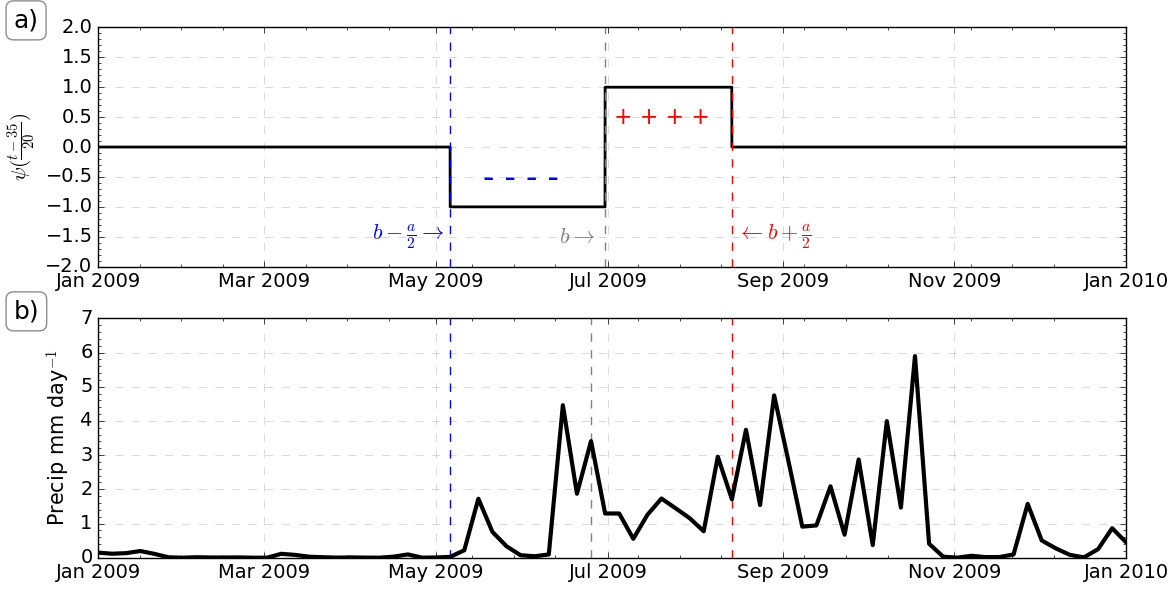
\includegraphics[width=\linewidth]{figures/wav1.png}
\caption[Haar wavelet exmaple]{ (a) Haar wavelet at a dilation $a=20$ and translation $b=35$, which is the 35rd pentad around June 22. The positive and negative parts of the wavelet are highlighted in red and blue, respectively. (b) CMAP precipitation in 2009 in the North American Monsoon [20-27$^\circ$N,110-103$^\circ$W]. }
\label{fig:wvt_f1}
\end{figure}


\begin{figure}[t!]
\centering
 %\noindent
 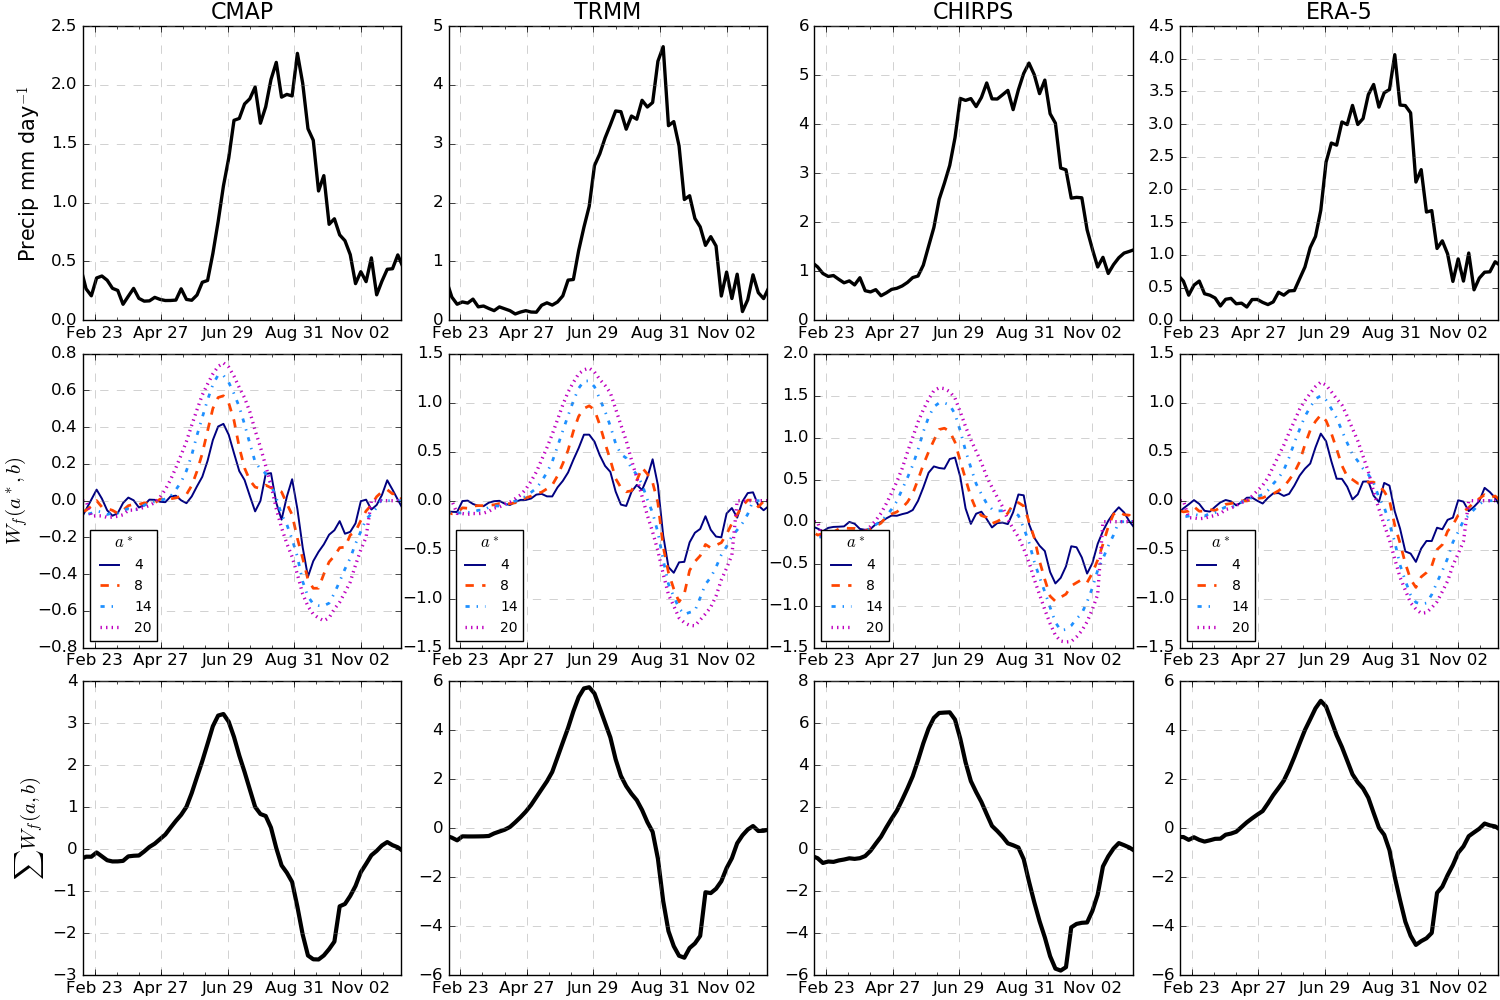
\includegraphics[width=\linewidth]{figures/wav_paperfig2.png}
\caption[Wavelet transform coefficient in North American Monsoon]{ (upper) Climatological pentad-mean precipitation in four different observational datasets in the North American Monsoon [19-35$^\circ$N,110-103$^\circ$W]. (middle) The wavelet transform coefficients (mm d$^{-1}$) for four different dilations $a$. (lower) The sum of the WT coefficients (mm d$^{-1}$) over dilations $a={4,8,14,20}$. }
\label{fig:wvt_f2}
\end{figure}

Figure \ref{fig:wvt_f1} shows the Haar wavelet and one year of observed precipitation in the North American Monsoon from the CMAP dataset. Figure \ref{fig:wvt_f1}a illustrates how the wavelet function compares the observed signal in the interval $ b < t \leq b+\frac{a}{2}$ with the values of the signal in the interval $b-\frac{a}{2} \leq t < b$ where $b$ in this case is a pentad time step. The WT coefficient for dilation $a=20$ pentads at the translation of $b=35$, i.e., pentad 35, is a measure of the precipitation difference between the sum of the observed rainfall 10 pentads after pentad 35 and the sum of the observed rainfall 10 pentads before pentad 35 as illustrated in Figure \ref{fig:wvt_f1}b.


Figure \ref{fig:wvt_f2} shows an example of the WT application using the observed climatological precipitation in the North American Monsoon in four different precipitation datasets.
The mean climatological rainfall rates (upper panel) differ in their peak summer rainfall rates but qualitatively show similarities in the start and end dates of the rainy season. 
The WT coefficients ($W_f(a,b)$ in the middle panel) for a small dilation $a=4$ are relatively noisy but show a clear maximum and minimum that correspond well with the maximum and minimum of longer dilations ($a=14,20$). The sum of these four coefficients at each translation or pentad $b$, highlight a maximum found around June 22 and a minimum found around September 21, which agree well with previous results of mean onset and retreat dates in the North American Monsoon  \citep[e.g.][]{arias2012,geil2013}.


\subsection{Identification of Monsoon Onset and Retreat}

Local maxima in the WT highlight positive steps in the precipitation time series with a coherent scale of $a$ pentad steps. This interpretation is then extended to diagnose monsoon onset. 
 The pentad ($b^*$) corresponding to the maximum of the sum of the transform over a set of scales is defined as monsoon onset (MO), i.e: 
\begin{equation}
MO=b^* \Leftrightarrow \sum_{a_0}^{a_f} W_f(a,b^*)=max\bigg(\sum_{a_0}^{a_f} W_f(a,b)\bigg).
\label{eq:mo}
\end{equation}

\noindent where $a_0$ and $a_f$ are the limits of the pentad scales, i.e., the dilation coefficients, $b^*$ is the pentad of maximum $\sum W_f(a,b)$ and the monsoon onset pentad.
Similarly, the monsoon retreat pentad is found at the minimum of the sum of the WTs, i.e.,

 \begin{equation}
MR=b^* \Leftrightarrow \sum_{a_0}^{a_f} W_f(a,b^*)=min\bigg(\sum_{a_0}^{a_f} W_f(a,b)\bigg).
\label{eq:mr}
\end{equation}

\begin{figure}[t!]
\centering
 %\noindent
 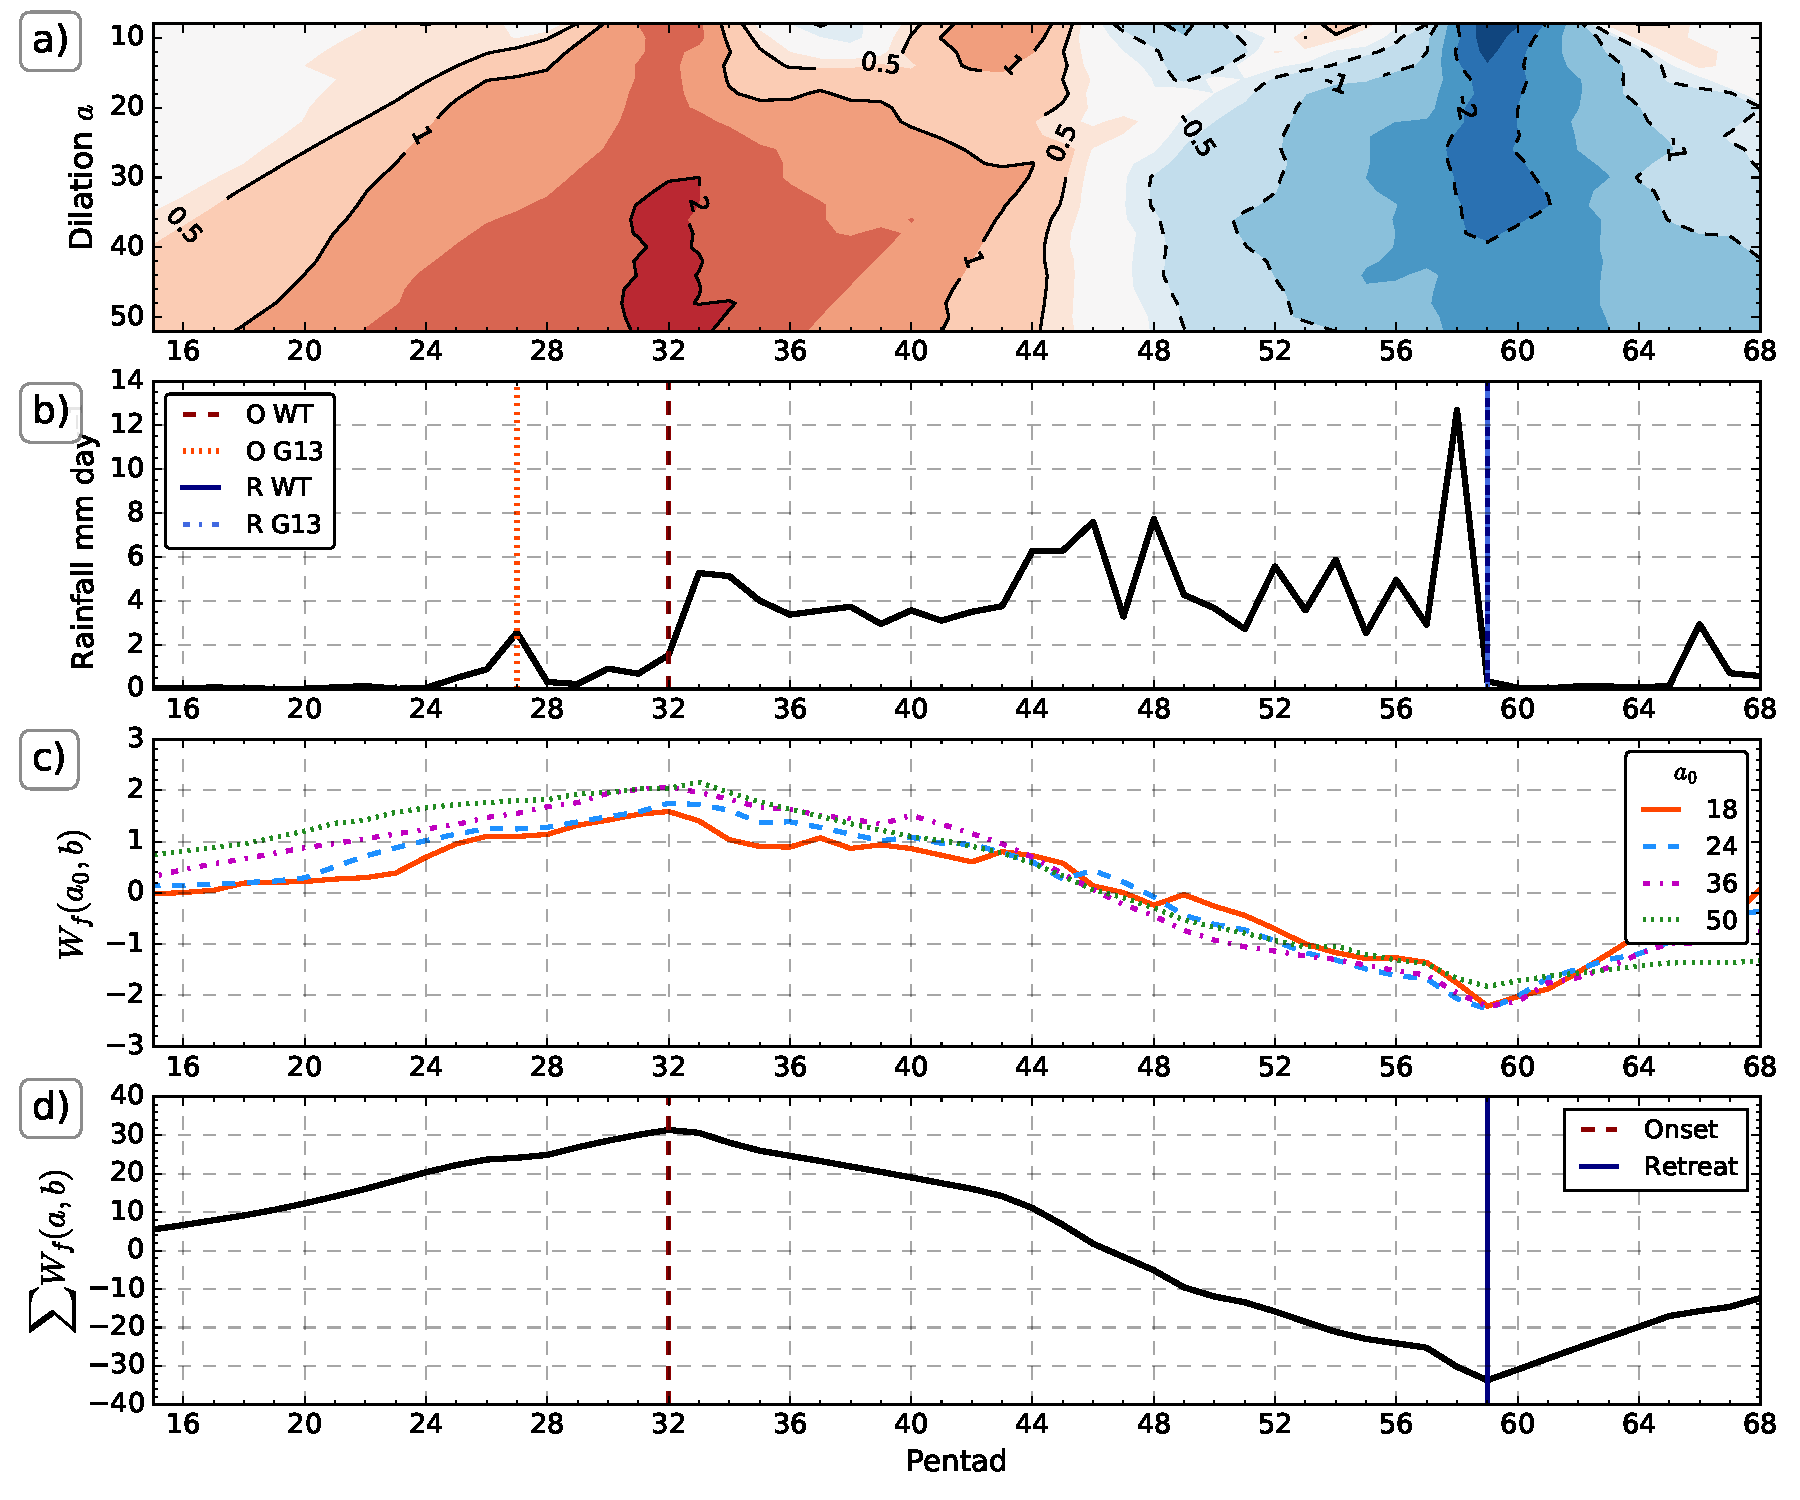
\includegraphics[width=\linewidth]{figures/wav_fig3.pdf}
\caption[Example determination of onset and retreat in TRMM]{ Example determination of monsoon onset and retreat dates for the North American Monsoon [20-27$^\circ$N,109-103$^\circ$W] in the TRMM dataset for 2009.
(a) WT coefficient matrix (mm d$^{-1}$) as a function of time and dilation coefficient $a$. The shading is from -3 to 3 mm d$^{-1}$  with an interval of 0.5 mm d$^{-1}$.
(b) Observed precipitation, the onset and retreat dates as determined by the WT method (dashed) and the threshold method of \cite{geil2013} (solid) are shown. Note that the date of retreat is diagnosed to be the same between the two methods.
(c) The WT coefficients for different dilations. (d) The sum of the WT ($\sum W_f(a,b)$) (mm d$^{-1}$); the maximum and minimum are shown in red and blue, representing onset and retreat pentads, respectively.  }
\label{fig:wvt_3}
\end{figure}

In other words, we seek to find monsoon onset and retreat using the maximum and minimum the wavelet power spectrum over a range of temporal scales.
Several sensitivity tests were performed with different dilation coefficients ($a$) in the different observational datasets, models and regions and a set or vector of dilation scales was found to be optimal. 
The set of dilation coefficients $\vec{a} = (28,30,\cdots, 54)$ was found to be robust, i.e., was able to capture the onset and retreat dates in all the datasets.

 Monsoon onset is defined as the maximum sum of wavelet coefficients, capturing positive gradients within the scales of 14 to 27 pentads (half of the elements of vector $a$ defined above). Monsoon Retreat has a similar definition, capturing the greatest negative gradient of precipitation over the same pentad scales.

For example, Figure \ref{fig:wvt_3} illustrates the method in the North American Monsoon in the TRMM dataset for 2009. Figure \ref{fig:wvt_3}a shows the WT coefficient matrix, showing the changes in precipitation for dilations ranging from 10 to 50. A clear signal of positive coefficients is observed between pentads 28 to 34  and a similar negative signal observed in pentads 56 to 60. Figure \ref{fig:wvt_3}b shows the time series of the observed precipitation, which suggests that monsoon onset occurs sometime between pentads 28 and 34. Observed rainfall rapidly decreases after pentad 59 suggesting that monsoon retreat can be diagnosed around this pentad.

\begin{figure}[t!]
 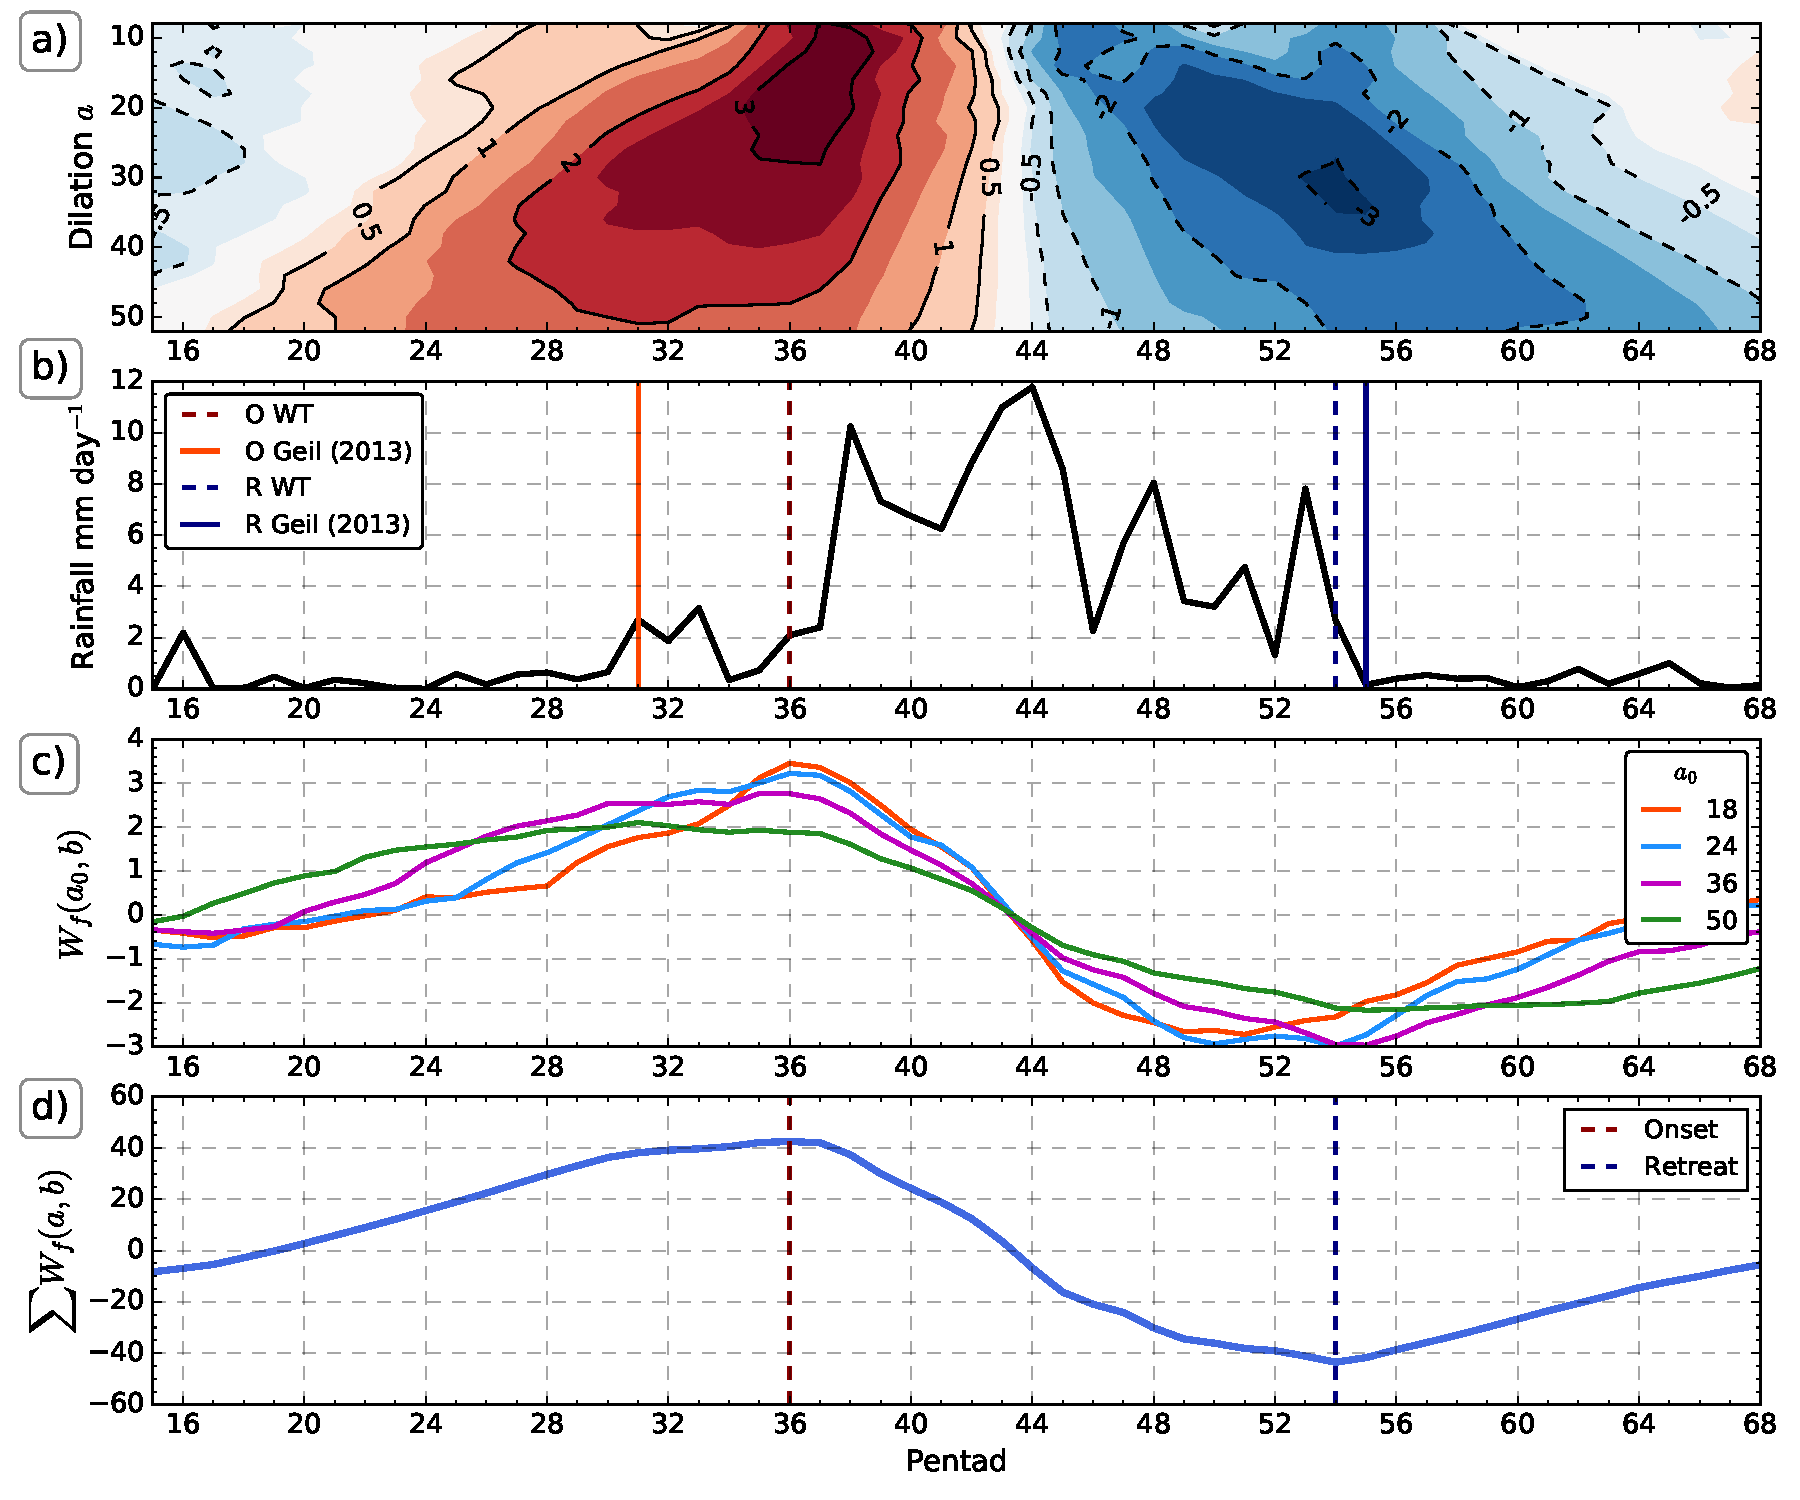
\includegraphics[width=\linewidth]{figures/nam_n216.pdf}
\caption[Example determination of onset and retreat in HadGEM3 N216]{ As in Figure \ref{fig:wvt_3}, but for a year (1875) in the HadGEMGC3.1 N216 pre-industrial control simulation.  }
\label{fig:s1_n216}
\end{figure}

 Figure \ref{fig:wvt_3}c shows the WT coefficients as a function of pentad for several dilations ($a_0$). The coefficients for all scales seem to follow a very similar behaviour, increasing during spring to reach a maximum around pentad 32 and thereafter decreasing to a minimum around pentad 59. When the sum of the wavelet transform coefficients across the dilations is computed (Figure \ref{fig:wvt_3}d) this behaviour becomes much clearer. The maximum and minimum are found at pentads 32 and 59, respectively and these pentads define the onset and retreat times. For comparison, the results from the method of \cite{geil2013} are shown in Figure \ref{fig:wvt_3}b, indicating that this method may have found an earlier onset. 
 
 As a proof of concept, Figure \ref{fig:s1_n216} shows a similar example using precipitation area-averaged in the same region but using model data from the piControl simulation of HadGEM3 GC3.1 N216. 
 The results show that the WT method can capture the onset and retreat dates with relatively high skill and that these dates are different from the dates computed using the method of \citetalias{geil2013}, with the threshold method suggesting an earlier onset and a later retreat. 

\subsection{Extension for Application to the MSD signal}




The wavelet method can be extended to characterise the shorter scale variations of precipitation of the MSD in Central America and the Caribbean. First, the monsoon onset and retreat dates are determined in the time series from the area-averaged precipitation in the MSD region via the approach described in the previous section. 
Once the onset and retreat dates are established, an additional wavelet analysis determines the dates in which the MSD starts and ends.
The onset and end of the drier period of the MSD can be found by computing the wavelet transform again but using smaller dilations and over a limited temporal range. In particular, the WT is only calculated in the 20 pentads before and after the dates defining monsoon retreat and onset, respectively. The MSD Onset (MSDO) and MSD End (MSDE) are defined as the minimum and maximum, respectively, of the sum of the wavelet transforms (equations \ref{eq:mo} and \ref{eq:mr}) using dilation coefficients $\vec{a^*} = (10,12,\cdots, 24)$.
The diagnosis of the onset and end of the MSD is algo robust to using other dilation coefficients of similar magnitude.

Figure \ref{fig:5} illustrates the use of the WT method to determine the dates of MSDO and MSDE for the precipitation of 2017 in ERA-5.
Figure \ref{fig:5}a depicts the wavelet covariant transform matrix, showing the $W_f$ coefficients for each dilation $a$ at each pentad $b$. The onset of rainfall is diagnosed around the time-steps of highest positive $W_f$ coefficients -- around pentads 24 to 32 for almost all dilations. These positive coefficients are followed by a period of negative values from pentad 32 to pentad 40, which represent the decrease in precipitation, or relative drought, in the midsummer. The MSD is followed by another period of positive coefficients from pentad 44 to pentad 52, illustrating the so-called second peak of precipitation and, finally, a period of negative coefficients associated with monsoon retreat.

\begin{figure}[t!]
\centering
 %\noindent
 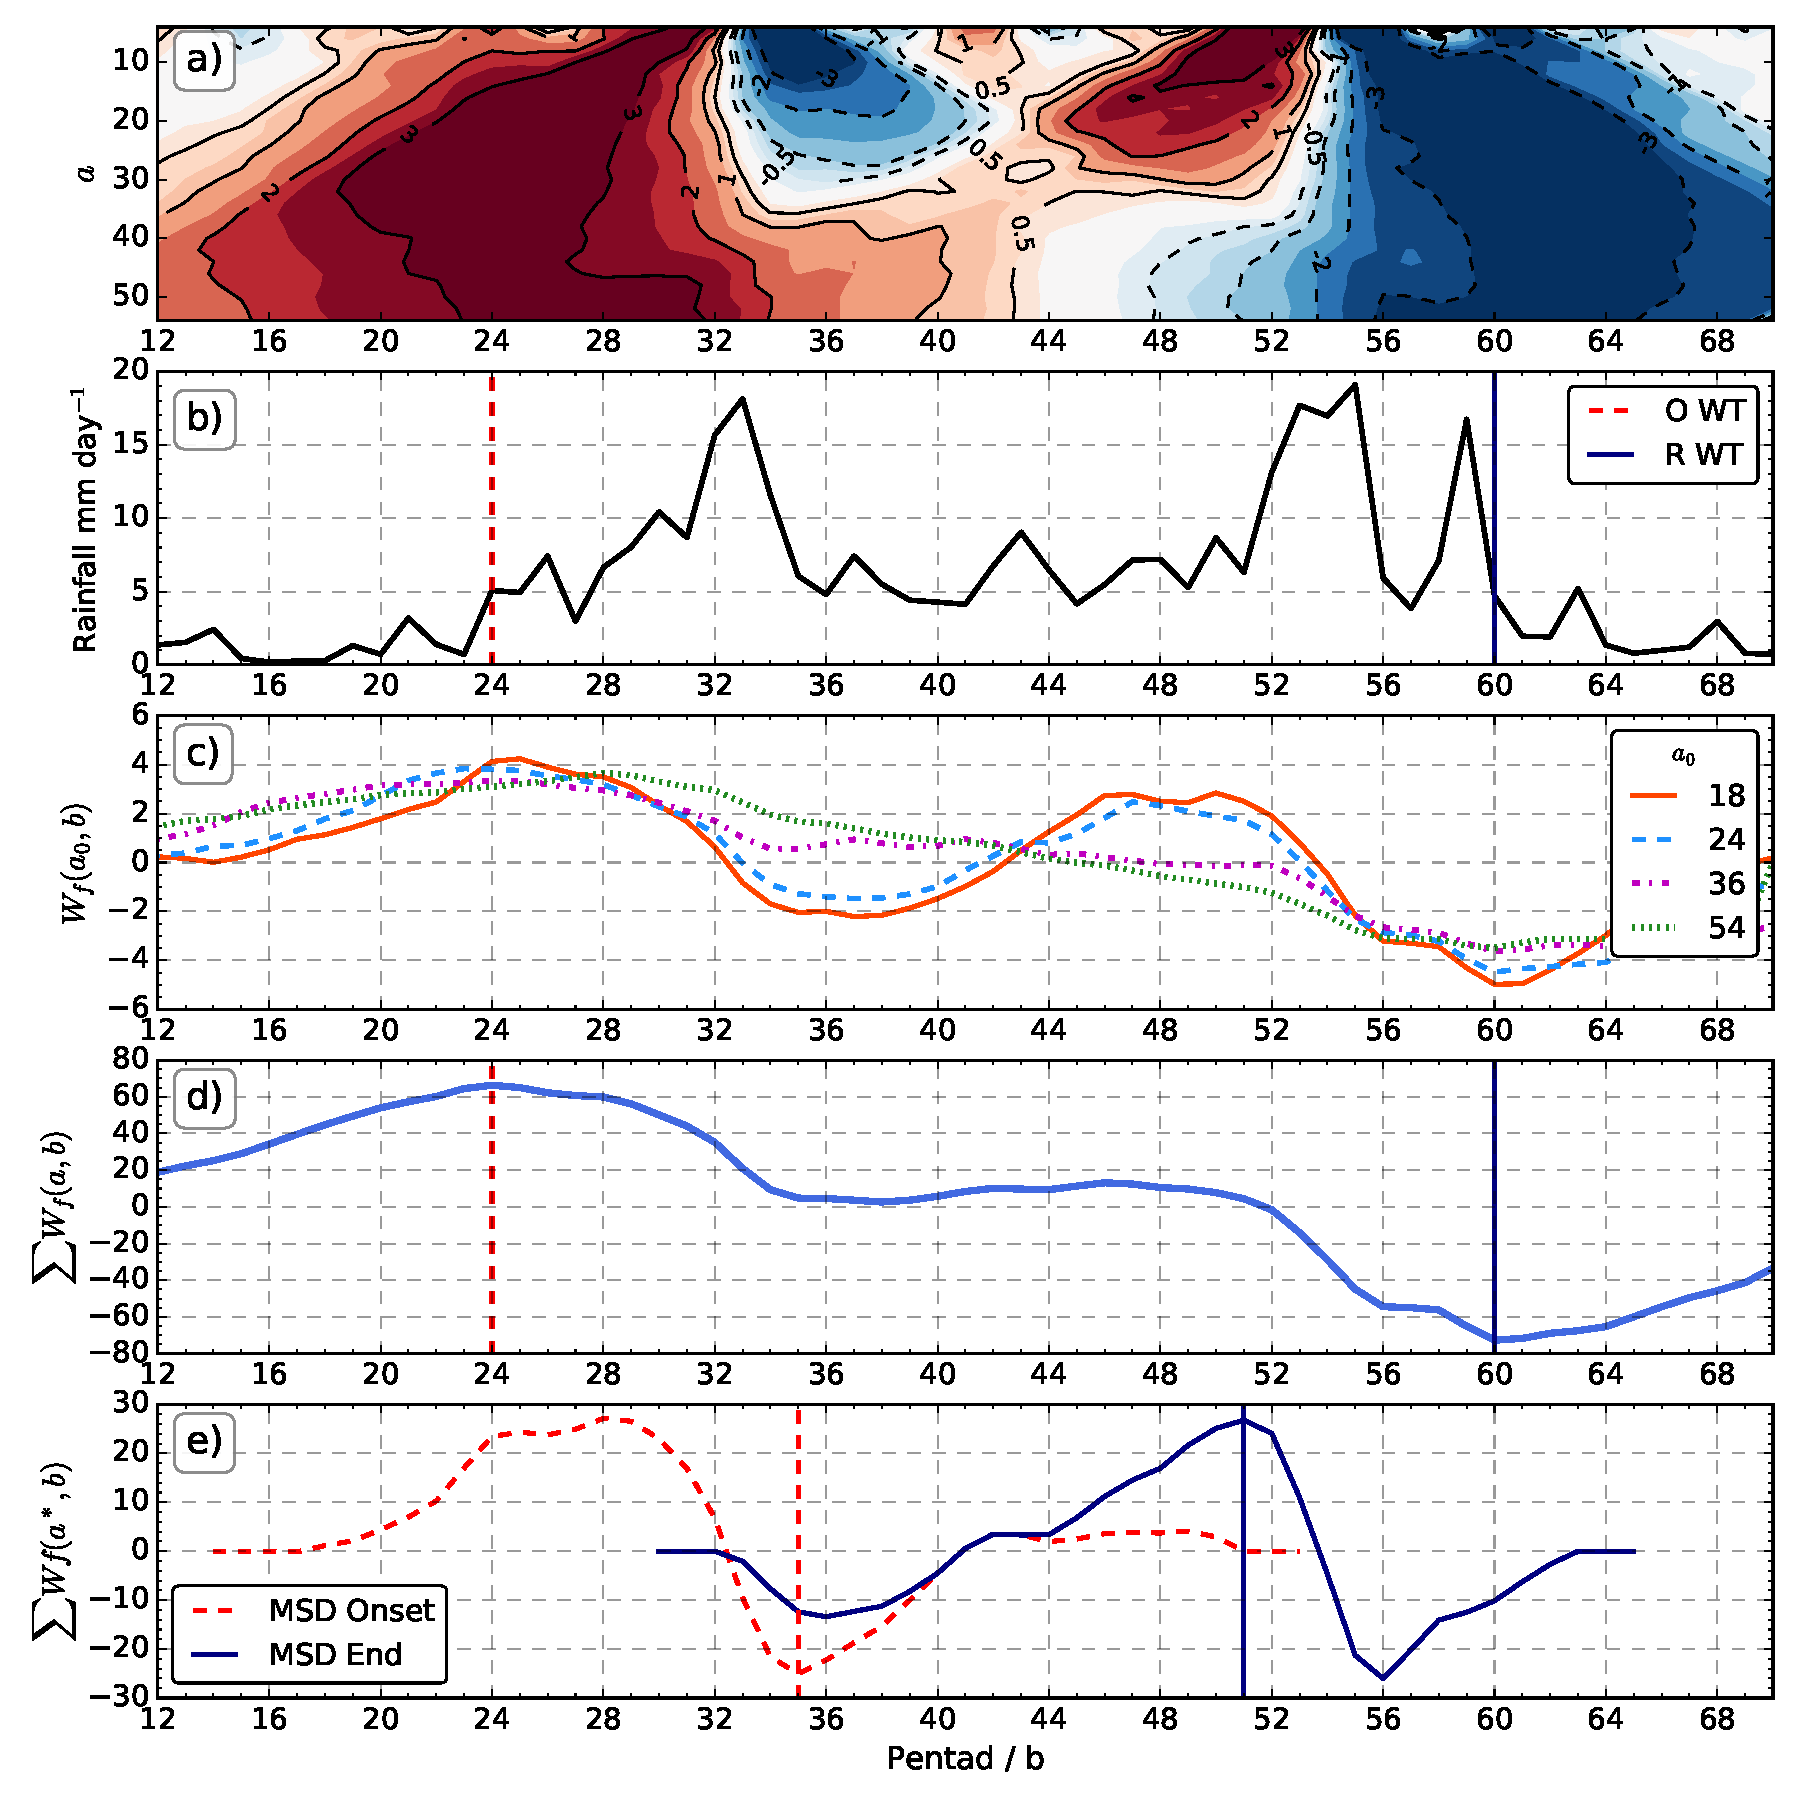
\includegraphics[width=\linewidth]{figures/wav_fig4.pdf}
\caption[Wavelet transform characterisation of Midsummer drought]{ Example characterisation of the MSD [11-19$^\circ$N,95-85$^\circ$W] using ERA-5 data for 2017. (a) Wavelet transform spectra, (b) observed precipitation with the onset and retreat pentads shown in red and blue, respectively. (c) Wavelet transform coefficients for four different dilations (mm d$^{-1}$). (d) The sum of the wavelet transform coefficients (mm d$^{-1}$) for $a={28,..,51}$. (e) The sum of $W_f(a,b)$ (mm d$^{-1}$) for dilation coefficients $a={12,..,24}$ showing the start (MSD Onset) and end (MSD End) of the midsummer drought. }
\label{fig:5}
\end{figure}

The coefficients of the wavelet transform ($W_f(a_0,b)$) for selected dilations $a_0$  (Figure \ref{fig:5}c) show that the smaller dilations are more sensitive to smaller scale variations in the time series and longer dilations better highlight the long-term change of the time series. For example $a_0=18$ shows signs of a MSD by showing two local maxima and two local minima, whereas $a_0=54$ only shows a local maximum and a local minimum associated with onset and retreat.

The maximum and minimum of the sum over all dilations (Figure \ref{fig:5}) depict the rainfall onset and retreat dates, respectively. The second wavelet transform $W_f(a^*,b)$ is computed over smaller dilation coefficients ($a^*$) near the onset and retreat dates as described above to highlight the MSDO and the MSDE.
Figure \ref{fig:5}e shows the sum of the wavelet transform coefficients  $W_f(a^*,b)$ and the pentad of the MSDO, 34, and MSDE, 49, corresponding to the minimum and maximum of the sum of these wavelet transform coefficients, respectively.

The strength of the MSD can be measured through the maximum and minimum sum of the coefficients $\sum W_f(a^*,b)$ used to define the start and end dates of the MSD.
For example, in Figure \ref{fig:5}e the minimum of the $\sum W_f(a^*,b)$ was -20\ mm\,d$^{-1}$ found at pentad 35 and an opposite local maximum of +20\ mm\,d$^{-1}$ at pentad 49. These two values, hereafter $coef1$ and $coef2$, provide a quantitative measure of the strength of the MSD for this year in this dataset and will be used to measure the spatial and temporal variability of the magnitude of the MSD in the different datasets.

\subsection{Comparative Methodologies}


For validation purposes, the wavelet transform method is compared with existing methods which determine onset and retreat in the North American and Indian monsoons. 
The threshold methods of \cite{geil2013} (hereafter G13) and \cite{arias2012} (hereafter A12) are compared to the results of the wavelet transform in the North American Monsoon.
\citetalias{geil2013} used a threshold of 1.3 mm day$^{-1}$ for at least 3 days for onset and 7 days for retreat for daily TRMM observations. This study, in contrast, analyses most of the data on the pentad-scale, so we adapt this method for TRMM to the same threshold value, but the onset pentad is the first pentad above the threshold whereas for retreat, we require rainfall to be below the threshold for two consecutive pentads.
 The method of \citetalias{arias2012} defines onset with two conditions. The first condition to find the onset pentad is that six out of the eight subsequent pentads must have rain-rates above the annual-mean climatological rainfall. The second condition is that at least six out of the eight previous pentads must be below the annual-mean climatological rainfall.
The opposite definition is used to determine the pentad of monsoon retreat. 

In relation for the Indian Monsoon region, a commonly used metric is the hydrological onset and withdrawal index (HOWI) which is based on moisture transport over the Arabian Sea \citep{fasullo2003,Sahana_2015,chevuturi2019}.
To compute the HOWI index, first, the vertically integrated moisture transport ($\chi$) is computed from daily ERA-5 data in the Arabian sea, as described by \cite{fasullo2003}, i.e.:

\begin{equation}
\chi=\frac{1}{g}\int_{p_0}^0 q \mathbf{V} dp,
\end{equation}
 \noindent where $g$ is the gravitational acceleration, $p$ are the pressure levels, $q$ is the specific humidity and $\mathbf{V}$ is the wind vector. The VIMT is then normalized using the transformation:

 \begin{equation}
 HOWI = 2 \bigg(\frac{\chi - min(\bar{\chi})}{max(\bar{\chi})-min(\bar{\chi})} \bigg)
 \end{equation}

 \noindent where $\chi$ is the unnormalized time series, $\bar{\chi}$ is the mean seasonal cycle of the unnormalized index and HOWI is the normalized index. The onset date is defined as the first day of each year where the HOWI index is greater than zero and the retreat date is the first day after the onset date that the HOWI index is negative \citep{fasullo2003,Sahana_2015}.
 The necessary daily data of moisture and wind speed on sufficient vertical levels to compute the HOWI index in the MOHC submissions to CMIP6 was not available, so the HOWI index can only be computed using ERA5 and will be compared to the WT method used on the observational gridded datasets.

\section{Results}

\begin{table}[b!]
% table caption is above the table
\caption{Mean (standard deviation) pentads of monsoon onset (O) and retreat (R) in the North American Monsoon [110$^\circ$-103$^\circ$W, 20$^\circ$-27$^\circ$N] for observational datasets, reanalysis and model output with the wavelet transform method WT, G13's and A14's method. Pentad 34 corresponds to the period between June 17-22 and pentad 54 to the period Sep 27 - Oct 1. The results from the WT method in the model experiments which are statistically different to both the CMAP and CHIRPS results at the 95\% confidence level, according to a Welch's t-test, are shown in bold. }
\label{tab:3}       % Give a unique label
% For LaTeX tables use
\begin{tabular}{p{2.2cm}p{1.765cm}p{1.765cm}p{1.765cm}p{1.765cm}p{1.7655cm}p{1.7655cm}}
\hline\noalign{\smallskip} \small
Dataset / Experiment & WT O 	& WT R 	& G13 O & G13 R & A12 O & A12 R \\ \hline
TRMM & 33.3 [$\pm$1.8] & 55.8 [$\pm$1.9] & 33.0 [$\pm$1.7] & 56.6 [$\pm$1.4] & 30.4 [$\pm$1.7] & 53.8 [$\pm$2.0]  \\
CMAP & 33.2 [$\pm$1.6] & 55.0 [$\pm$2.1] & 36.0 [$\pm$3.3] & 55.7 [$\pm$1.8] & 31.7 [$\pm$3.0] & 54.5 [$\pm$3.3]   \\
CHIRPS & 32.5 [$\pm$1.5] & 54.7 [$\pm$1.9] & 33.6 [$\pm$1.7]& 56.1 [$\pm$1.4] & 30.1 [$\pm$1.7] & 53.6 [$\pm$2.5]   \\
ERA-5 & 33.5 [$\pm$1.8] & 55.5 [$\pm$2.0] & 33.6 [$\pm$1.8]& 56.4 [$\pm$1.4] & 30.9 [$\pm$1.7] & 53.3 [$\pm$2.3]   \\
GC3 N216-pi  & 33.7 [$\pm$2.0] & 55.1 [$\pm$1.8]& 32.6 [$\pm$2.5] & 55.9 [$\pm$2.3] & 32.4 [$\pm$2.5] &53.8 [$\pm$3.8]  \\
GC3 N96-pi & 33.7 [$\pm$2.2] & 55.0 [$\pm$2.1] & 32.7 [$\pm$2.9] & 56.3 [$\pm$2.0] & 31.9 [$\pm$2.6] & 54.1 [$\pm$4.1]  \\
GC3-hist & 33.8 [$\pm$2.3] & 55.1 [$\pm$2.1]& 33.3 [$\pm$2.9] & 56.0 [$\pm$2.2] & 31.9 [$\pm$2.6] & 53.7 [$\pm$4.0]  \\
UKESM-pi & \bf{34.5} [$\pm$2.1] & 54.8 [$\pm$2.1] & 34.1 [$\pm$2.9] & 56.1 [$\pm$1.9] & 33 [$\pm$2.6] & 53.9 [$\pm$4]   \\
UKESM-hist & \bf{34.3} [$\pm$2.2] & 54.3 [$\pm$2.2]& 34.4 [$\pm$3.2] & 55.6 [$\pm$2.1] & 33.1 [$\pm$3.0] & 53.2 [$\pm$4.2] \\
%\noalign{\smallskip}\hline\noalign{\smallskip}
%number & number & number \\
%number & number & number \\
%\noalign{\smallskip}\hline
\end{tabular}
\end{table}


The monsoon onset and retreat dates were determined for each year in each observational and model dataset for the Indian, North American and MSD regions using the methods described in the previous section. The calculations were performed for area-averaged precipitation time series representative of the core regions defining these monsoons. Calculations were also made at grid-box scales to illustrate the spatial distribution of the onset and retreat dates. 


\subsection{The North American Monsoon}






Table \ref{tab:3} shows the mean onset and retreat dates estimated using the \citetalias{geil2013}, \citetalias{arias2012} and WT methods for precipitation time series averaged over the North American monsoon.
The table reports the results for three observational datasets, ERA-5 reanalysis and five climate model experiments.
The observations  agree that the onset date is found at pentad 33 (around June 15), according to the WT and the method by \citetalias{geil2013}.
However, the method of \citetalias{geil2013} reports a mean retreat date that is one pentad later than the WT method, i.e., around October 7th for G13 method and October 2nd for the WT.
The method by \citetalias{arias2012} disagrees with \citetalias{geil2013} and the WT methods for both onset and retreat mean pentads, in both cases finding an earlier onset (pentad 30) and retreat (pentad 54) for all the observational datasets. 

\begin{figure}[t!]
\centering
 %\noindent
 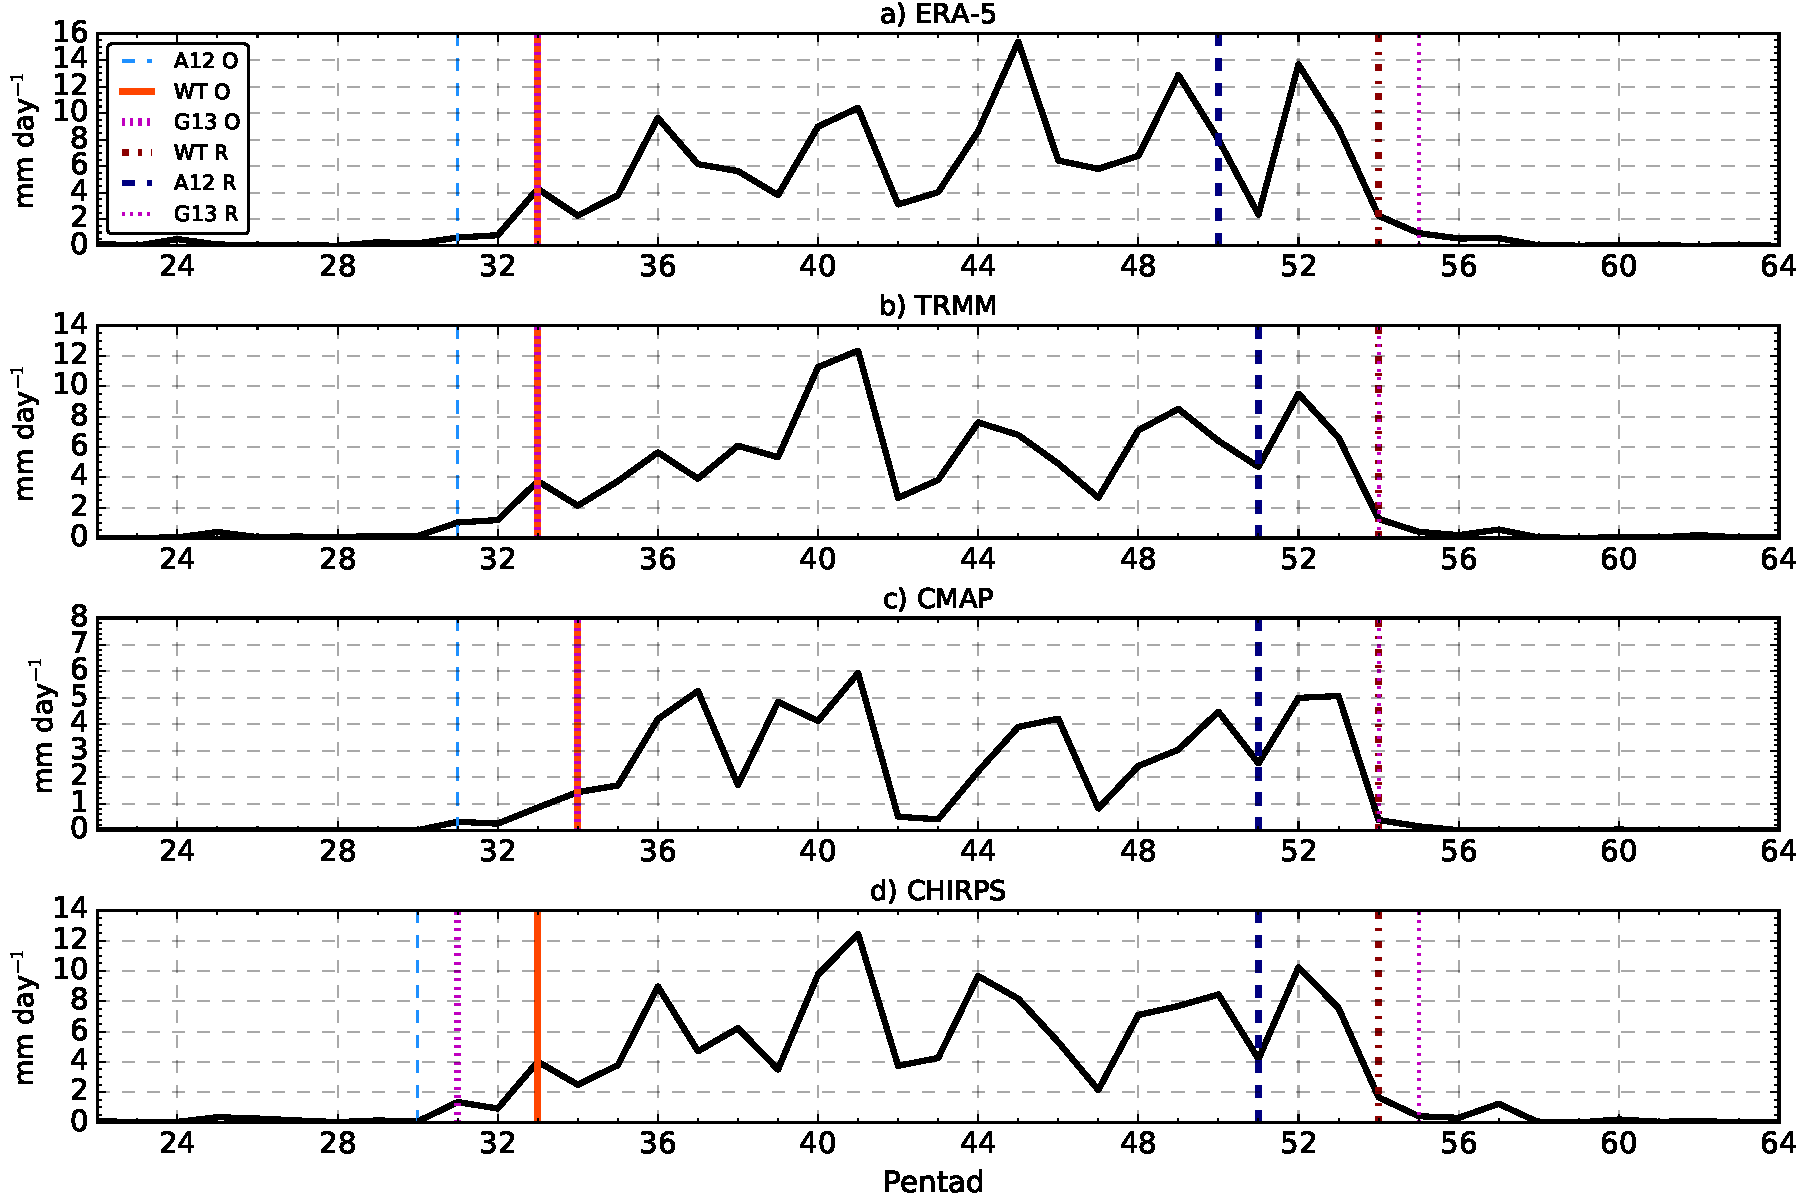
\includegraphics[width=\linewidth]{figures/wav_fig5.pdf}
\caption[Comparison of methods in 2010 in the North American Monsoon]{  Pentad-mean precipitation for the North American Monsoon in 2010 in four precipitation datasets showing the onset and retreat pentads as diagnosed by the WT, the A12 and G13 methods. The area used to average the precipitation is illustrated in in Figure \ref{fig:wav_fig6}b).} 
\label{fig:wav_compari}
\end{figure}


\begin{figure}[t!]
\centering
 %\noindent
 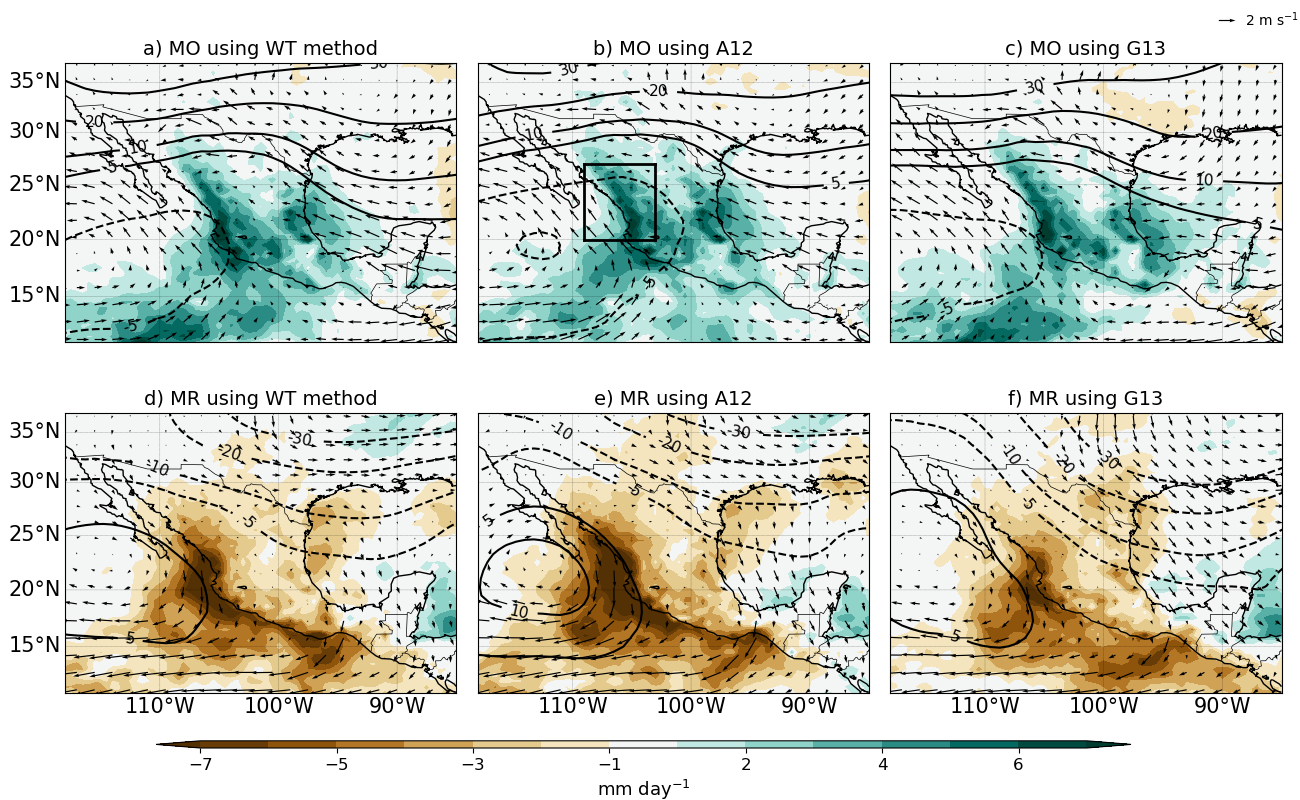
\includegraphics[width=\linewidth]{figures/wav_fig6.png}
\caption[Precipitation anomalies during North American monsoon onset]{  Precipitation (color contours), low level wind at 850-hPa and geopotential height (line contours) at 500 hPa anomalies for (a, b, c) the difference between the 10 days after monsoon onset and 10 days prior to onset (MO) using onset dates from (a) the WT (b) \cite{arias2012} and (c) \cite{geil2013}. (d, e, f) are as in (a, b, c) but for monsoon retreat. The data and dates are obtained from ERA-5, and the area for the average is shown in the box in b). }
\label{fig:wav_fig6}
\end{figure}

The climate models reasonably represent the mean onset and retreat dates, as only the onset dates from both experiments of UKESM1 are statistically different to the results of CMAP and CHIRPS. The similiarities in onset and retreat dates confirm that the seasonal cycle in the North American monsoon is very well represented by these models, as suggested by chapter \ref{ch:4-ams}. In the results of the simulations, \citetalias{arias2012} also produces an earlier onset and retreat dates when compared to the other two methods of about 1.5 pentads, but this difference is within the uncertainty range given by the interannual variability of the model data which is largest for  \citetalias{arias2012}.  

Figure \ref{fig:wav_compari} compares the estimated onset and retreat dates using the three methods for the 2010 North American Monsoon  using the three observational datasets and ERA5. \citetalias{arias2012} shows an earlier onset and retreat in all the datasets compared with the WT and \citetalias{geil2013} which agree in almost every dataset. The WT method is the only method that estimated the same retreat date for all the four datasets and the same onset date in three of the four datasets, with the CMAP datasets showing an onset date one pentad later than the others. % delayed by only one pentad. 

\begin{figure}[t!]
\centering
 %\noindent
 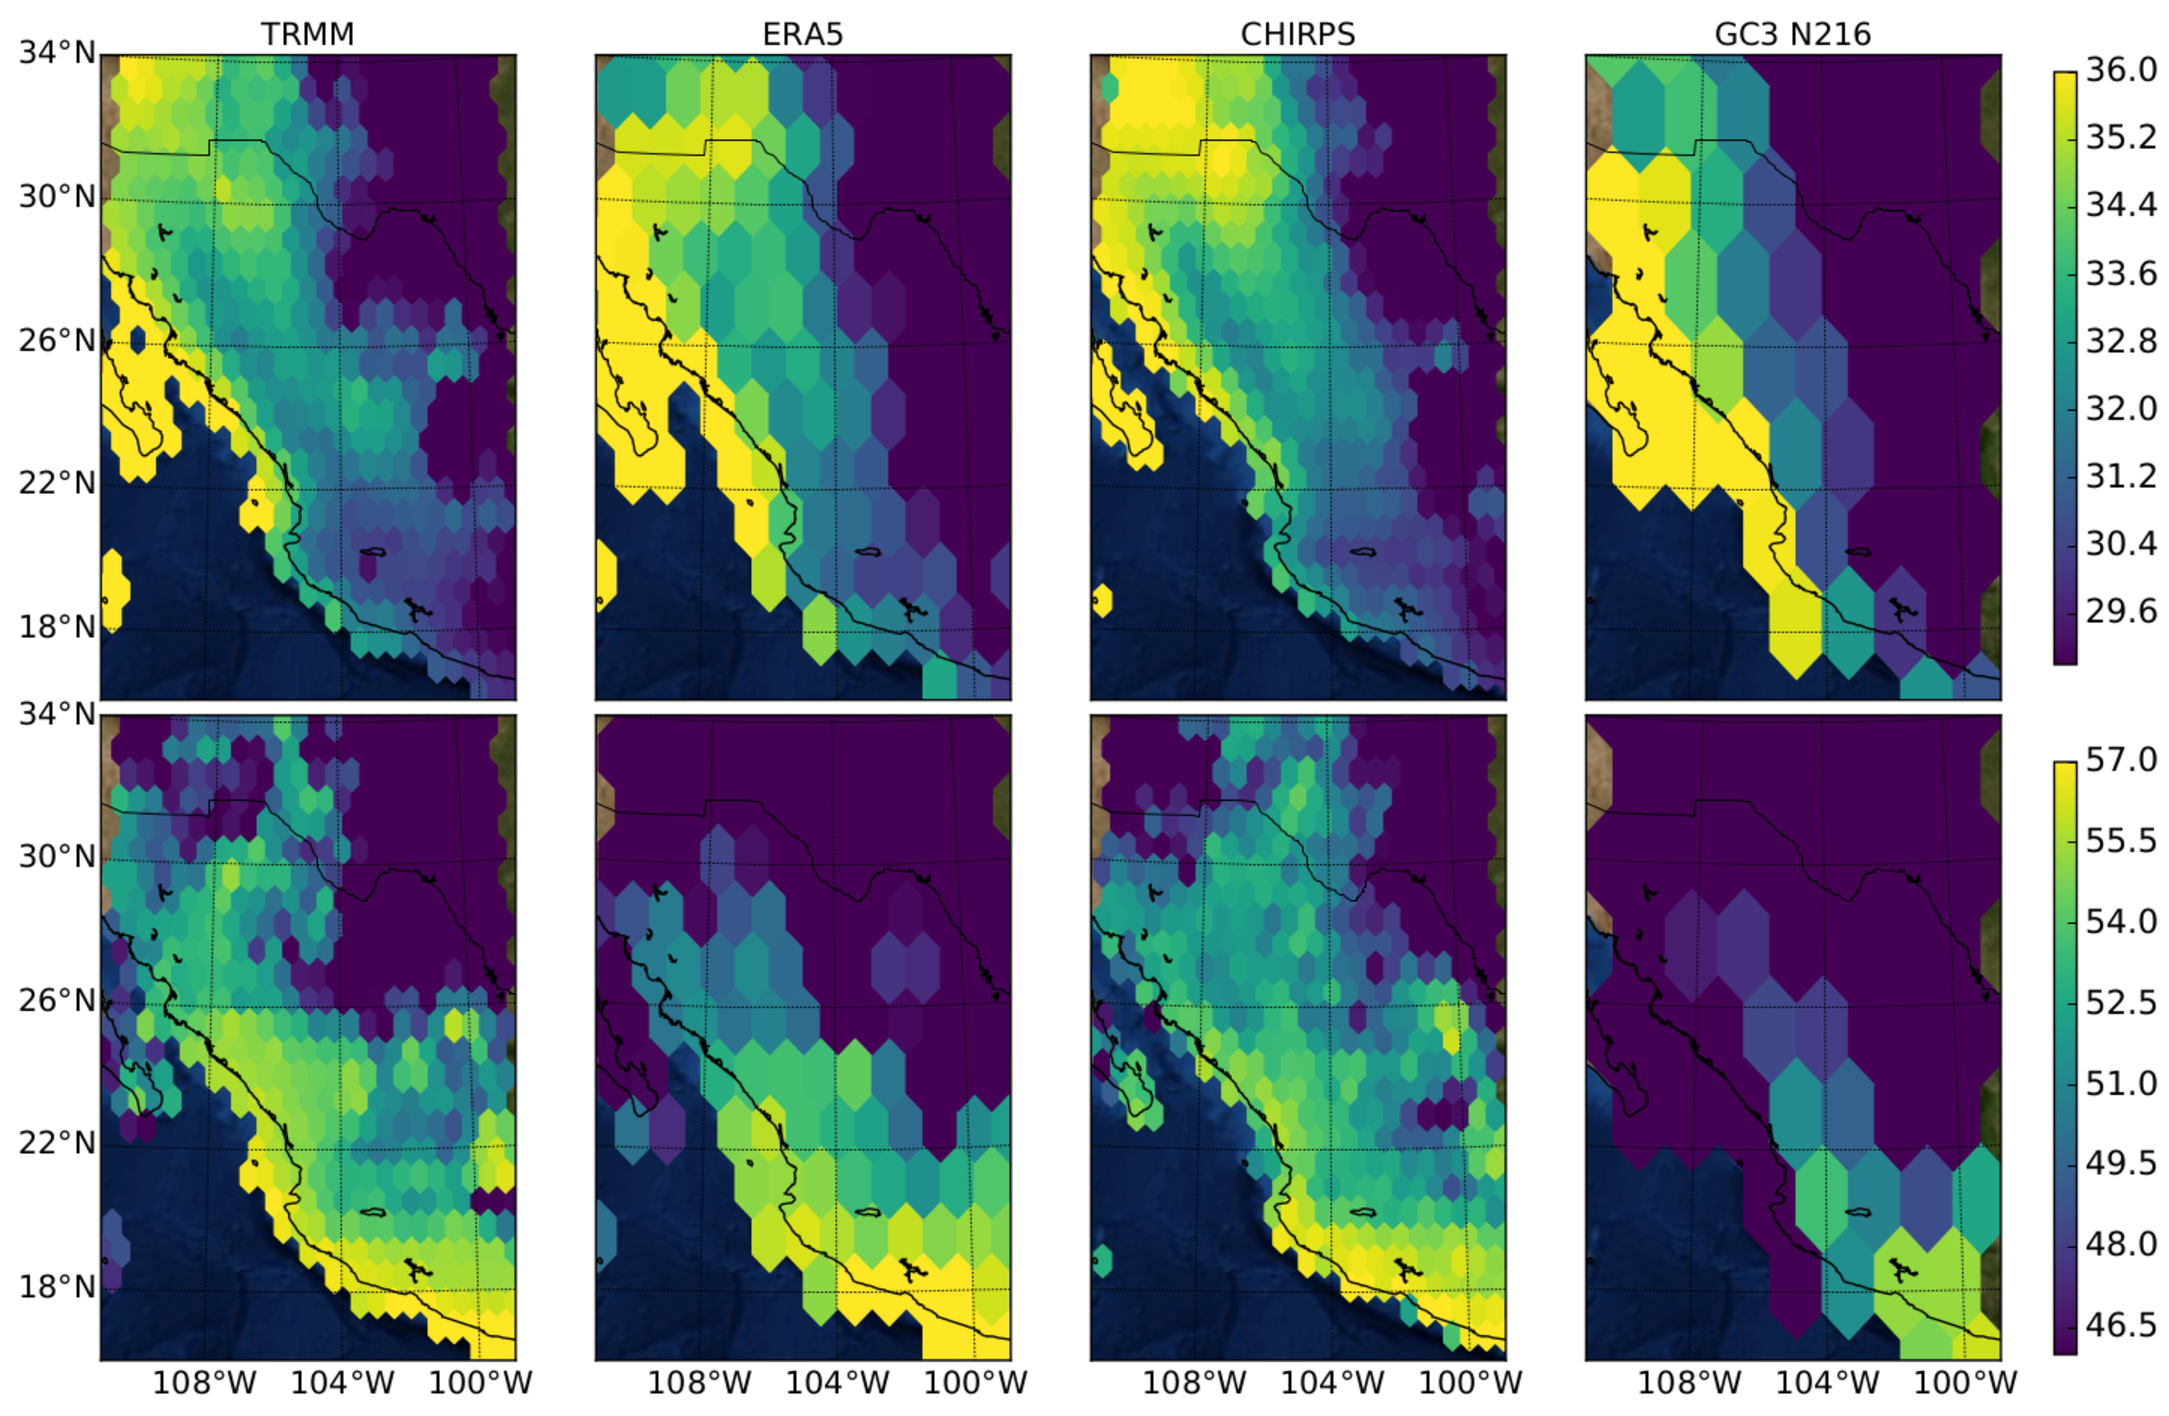
\includegraphics[width=\linewidth]{figures/map_nam_wav.pdf}
\caption[Onset and retreat spatial distribution in North American Monsoon]{ Rainfall onset (upper) and retreat (lower) mean pentads in the North American Monsoon for observations and a climate model output using the WT method.  }
\label{fig:nam_map}
\end{figure}

The meteorological changes associated with onset and retreat of the North American Monsoon  (Figure \ref{fig:wav_fig6}) are illustrated as the composite differences of the precipitation, wind and geopotential changes 10 days prior to and after onset and retreat. These changes to the circulation and precipitation are reasonably similar for all the three methods. The impact of monsoon onset in precipitation is diagnosed to be sligthly stronger by \citetalias{arias2012} compared to WT or \citetalias{geil2013}. 
The WT method shows a very similar pattern and magnitud of the circulation and precipitation anomalies of onset and retreat when compared to the other two methods. The method by \citetalias{geil2013} produces the weakest anomalies, particularly of precipitation whereas the method by \citetalias{arias2012} produces the strongest precipitation and geopotential anomalies, particularly at retreat.

Figure \ref{fig:nam_map} shows the spatial distribution of the mean onset and retreat dates in the North American Monsoon region for various datasets.
There is high agreement between TRMM, CHIRPS and ERA5 on the spatial pattern of mean onset and retreat dates.
Onset in western Mexico is around pentad 31 (around June 1st), whereas in Chihuahua and Sonora the rainy season begins shortly after pentad 35 (June 22).
The pattern in the medium-resolution simulation GC3 N216 piControl is consistent with observations, particularly during onset.  However, the spatial pattern of the mean retreat dates in the northern regions of the monsoon show an earlier than observed retreat, possibly associated with the dry bias in this region in these models (see chapter \ref{ch:4-ams}).

\subsection{The Indian Monsoon}
\begin{table}[b!]
% table caption is above the table
\caption{Mean (standard deviation) pentads of monsoon onset (MO) and retreat (MR) in the Indian Monsoon using the WT method on observed, reanalysed and modelled time series as well as for the HOWI index. The region over which precipitation was area-averaged for the WT method was [75$^\circ$-83$^\circ$E, 18$^\circ$-24$^\circ$N]. The mean onset and retreat dates that are significantly different to the 99\% confidence level to the CMAP dataset are shown in bold.  }
\label{tab:3a}       % Give a unique label
% For LaTeX tables use
\begin{tabular}{p{4cm}p{3.5cm}p{3.5cm}}
\hline\centering{\smallskip}
Dataset & MO 	& MR 	\\ \hline
TRMM & 31.6 [$\pm$1.8] & 53.2 [$\pm$1.9]   \\
CMAP & 31.8 [$\pm$1.6] & 53.3 [$\pm$2.6]   \\
CHIRPS & 31.5 [$\pm$1.4] & 53.4 [$\pm$1.9]    \\
ERA-5 & 31.8 [$\pm$1.9] & 52.7 [$\pm$2.6]    \\
GC3 N216-pi  & {\bf34.4} [$\pm$1.3] & {\bf 50.5} [$\pm$1.9] \\
UKESM-pi & {\bf36.1} [$\pm$3.1] & {\bf 51.9} [$\pm$3.2]   \\
UKESM-hist & {\bf36.0} [$\pm$3.9] & {\bf51.8} [$\pm$3.3]   \\
GC3 N96-pi & {\bf35.5} [$\pm$1.8] & {\bf51.8} [$\pm$2.3]  \\
GC3-hist & {\bf35.7} [$\pm$2.1] & {\bf51.5} [$\pm$2.8]  \\
HOWI (ERA5) & {\bf29.5} [$\pm$2.3] & {\bf49.3} [$\pm$2.4]
%GC3.1 N216  & 33.4 [$\pm$3.1] & 56.1 [$\pm$2.5]  \\
%GC3 hist & 34.5 [$\pm$7.2] & 56.4 [$\pm$7.3]   \\
%UKESM hist & 35.2 [$\pm$2.3] & 55.1 [$\pm$8.8] \\
%\noalign{\smallskip}\hline\noalign{\smallskip}
%number & number & number \\
%number & number & number \\
%\noalign{\smallskip}\hline
\end{tabular}
\end{table}

Table \ref{tab:3a} compares the mean onset and retreat dates of the Indian Monsoon as computed from the HOWI index using ERA5 data, and the WT used for gridded precipitation datasets.
The onset and retreat dates from the HOWI index were converted from the daily to the pentad-scale to compare with the WT. The mean onset date for the HOWI index is May 27th between pentads 29 and 30, and retreat is between pentads 49 and 50, around September 3rd. The mean onset date found using the WT method for the four observational datasets was pentad 32, about two pentads later than the HOWI index. The mean retreat date for the WT method (pentad 53) was two pentads later than the HOWI results.

\begin{figure}[t!]
\centering
 %\noindent
 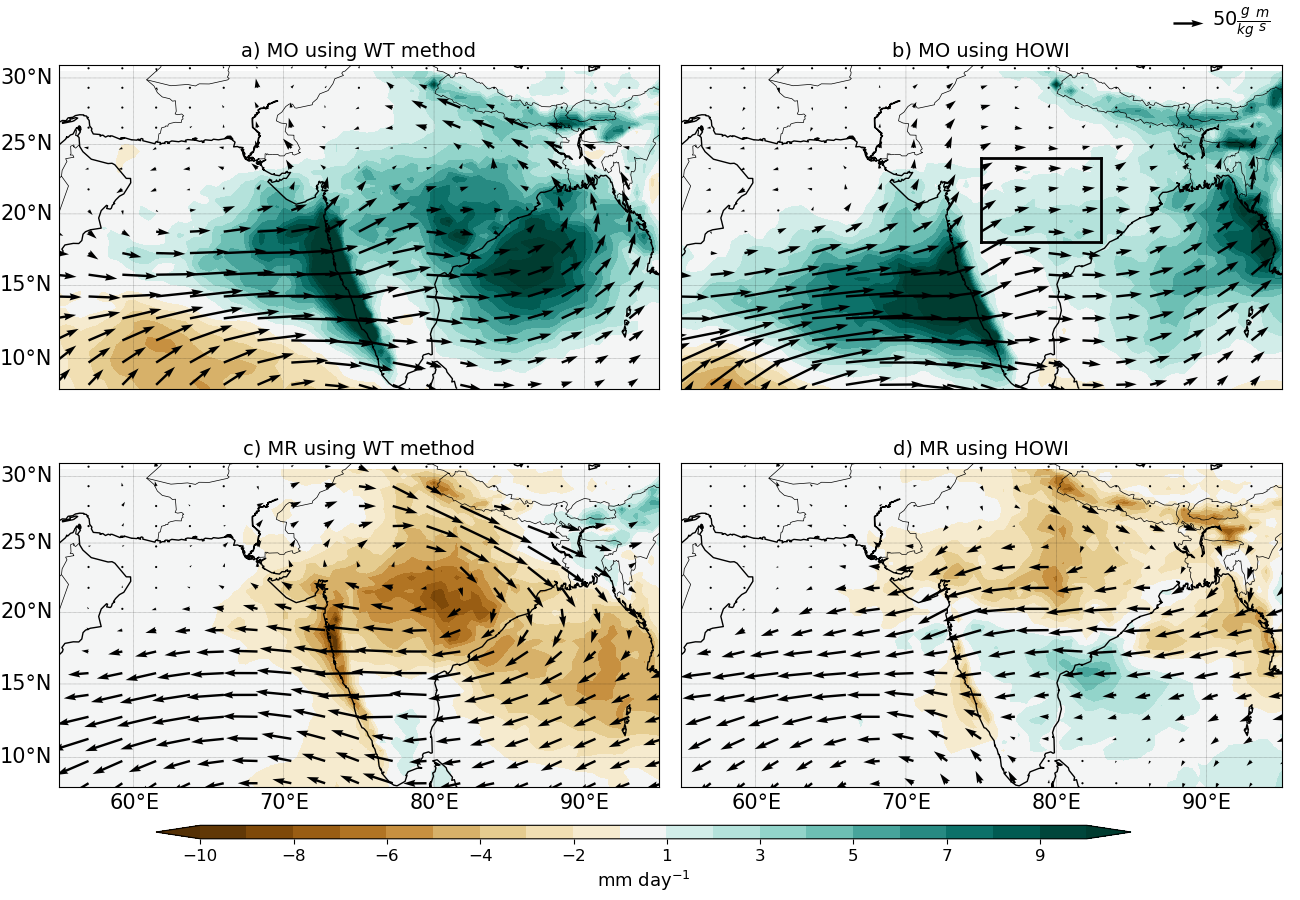
\includegraphics[width=0.95\linewidth]{figures/wav_fig8.png}
\caption[Precipitation anomalies during Indian monsoon onset]{  Precipitation anomalies (color contours) and the moisture flux vectors calculated from the product of specific humidity ($q$) and wind ($\vec{u}$) at 850 hPa. (a, b) shows the difference between the 10 days after monsoon onset and 10 days prior to MO using (a) the WT and (b) the dates estimated using the HOWI index. (c, d) are as defined in (a, b) but for MR. The dates are calculated from ERA5 data averaged over the box in panel b). }
\label{fig:wav_fig8}
\end{figure}

Overall, the models exhibited later than observed onset (+4 pentads) and earlier retreat  (-2 pentads) dates. The differences between the hydrological determination of onset and retreat dates, through HOWI, and the WT method on gridded precipitation datasets is statistically significant, according to a Welch's t-test comparing the HOWI and all the gridded datasets. These differences may be due to the different regions where each method is defined, i.e., HOWI is defined over the whole of the Arabian Sea where an earlier onset would be expected when compared to rainfall over mainland India, where the WT method was applied. 

\begin{figure}[t!]
\centering
 %\noindent
 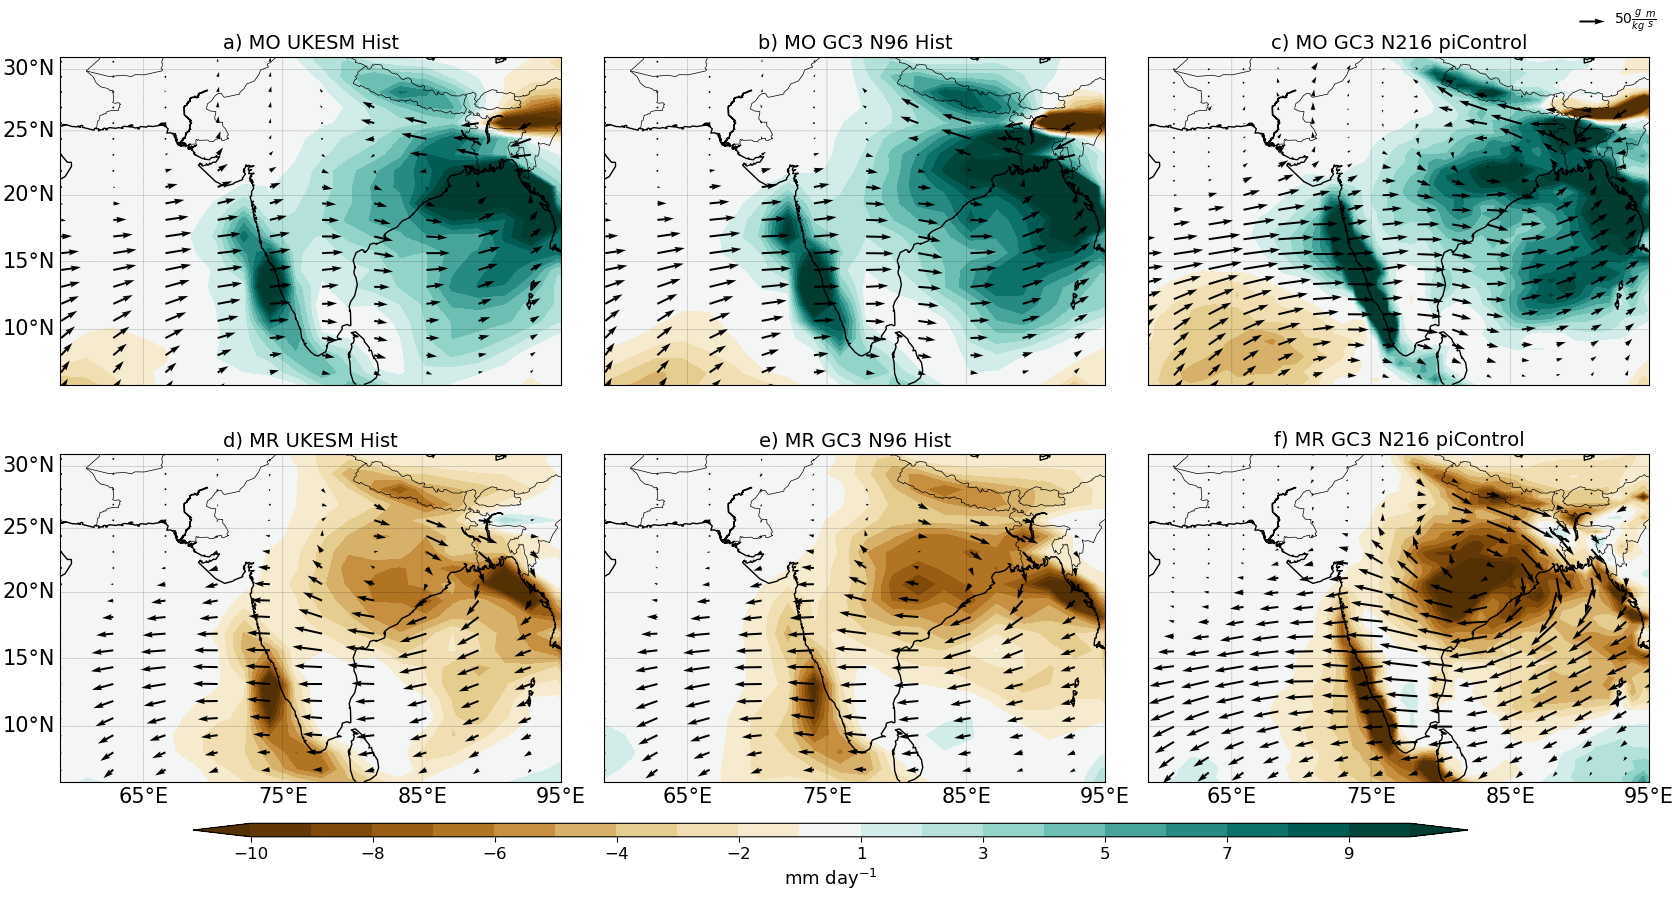
\includegraphics[width=\linewidth]{figures/ind_models.png}
\caption[Indian monsoon precipitation anomalies associated with onset]{ As in Figure \ref{fig:wav_fig8} but showing onset and retreat for three different climate model experiments: (a, d) UKESM1 historical, (b, e) HadGEM3 GC3.1 N96 historical, (c, f) HadGEM3 GC3.1 N216 piControl.   }
\label{fig:indmodels}
\end{figure}

Figure \ref{fig:wav_fig8} shows the differences between the WT (based on ERA5 precipitation) and HOWI methods in their characterisation of the meteorological changes associated with onset and retreat. 
The comparison of precipitation and moisture fluxes at 850 hPa anomalies 10 days prior to and following monsoon onset and retreat show that the HOWI index better captures the moisture transport in the Arabian Sea whereas the WT method best captures precipitation differences over mainland India. The HOWI index characterisation of the moisture flux in the Arabian Sea may be out-of-phase with precipitation over mainland India, and this lag could possibly explain some of the results of Table \ref{tab:3a}.


 The WT method is also able to capture onset and retreat dates and the associated anomalies within the climate model output. Figure \ref{fig:indmodels} shows the precipitation and moisture transport anomalies around the onset and retreat of the Indian monsoon in three different climate model experiments. While the models show significant biases in the timings of the monsoon, according to a Welch's t-test (Table \ref{tab:3a}), the patterns of rainfall and moisture transport anomalies to the observations around both onset and retreat agree well with reanalysis.

\begin{figure}
\centering
 %\noindent
 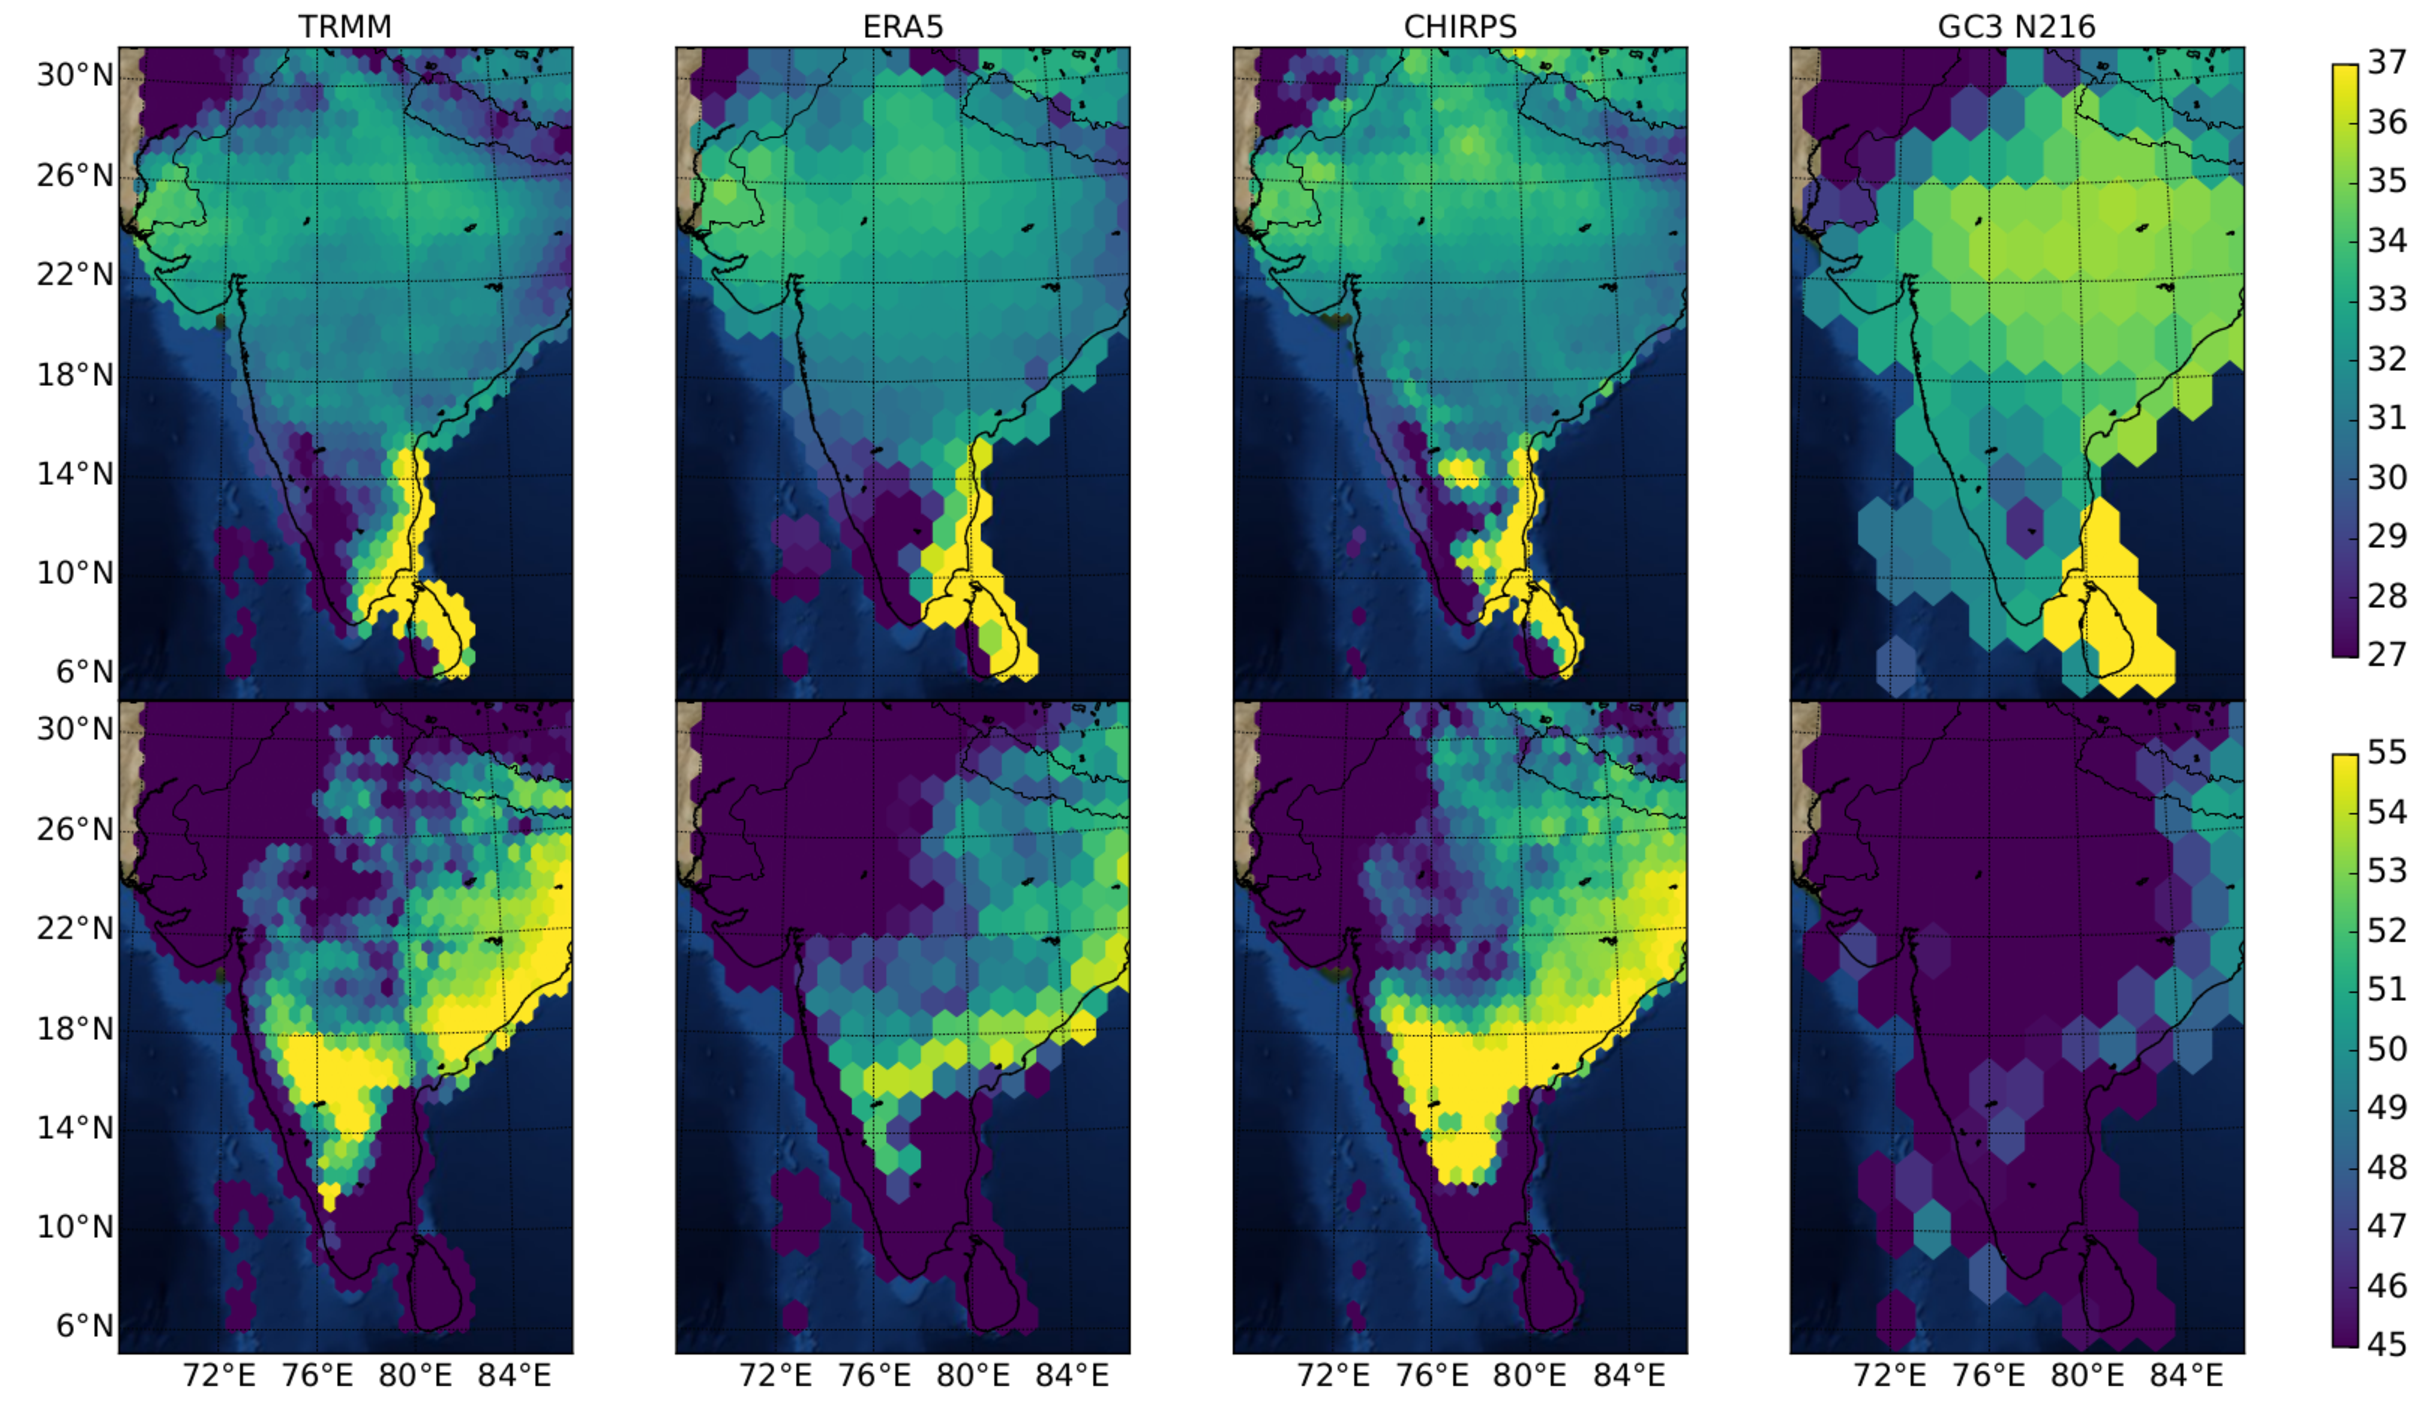
\includegraphics[width=\linewidth]{figures/wav_fig9.pdf}
\caption[Onset and retreat dates spatial distribution in Indian monsoon]{ As in Figure \ref{fig:wav_fig6} but for the Indian Monsoon.  }
\label{fig:wav_fig9}
\end{figure}

The spatial distribution of the mean onset and retreat dates of the Indian monsoon as characterized by the WT method (Figure \ref{fig:wav_fig9}) shows that the mean onset and retreat dates vary greatly spatially on the southern tip of the subcontinent. While most of northern India has a mean onset date around pentad 33, the western coast shows an earlier onset by about one or two pentads. There is high agreement in the onset date between the three observational datasets and the reanalysis over mainland India and between TRMM and ERA5 over the western coast of India. The earliest onset is found on the western coast around pentad 25-27 and extending to central India by pentad 31. 
The GC3 N216 simulation, however, shows a later onset than observed by about two pentads in most regions. In contrast, the spatial pattern for the mean retreat date shows higher spatial variability between the western and eastern coasts of India. CHIRPS shows the latest retreat dates over the south-central states when compared to TRMM and ERA-5. 

\subsection{The midsummer drought}

\begin{table}
% table caption is above the table
\caption{Mean pentads of monsoon onset (MO), rainfall retreat (MR), MSD Onset (MSDO) and MSD End (MSDE) in the MSD region [11-19$^\circ$N, 95-85$^\circ$W, illustrated in Figure \ref{fig:wav_fig11}a.] estimated through the WT method. Pentad 35 corresponds to the period between June 22-27 and pentad 52 to the period Sep 13-18. The model dates shown in bold are statistically different from CMAP and CHIRPS results to the 99\% confidence level according to a Welch's t-test. }
\label{tab:4}       % Give a unique label
% For LaTeX tables use
\begin{tabular}{p{2.35cm}p{1.7cm}p{1.7cm}p{1.7cm}p{1.7cm}p{2.1cm}p{1.925cm}}
\hline\noalign{\smallskip}
Dataset & MO & MR & MSDO & MSDE & coef1 & coef2  \\ \hline
TRMM & 25.8 [$\pm$2.2] & 61.6 [$\pm$3.1] & 35.9 [$\pm$2.4] & 49.0 [$\pm$4.1] & -9.5 [$\pm$4.2] & 10.4 [$\pm$5.4]  \\
CMAP & 26.7 [$\pm$1.9] & 60.6 [$\pm$3.3] & 36.5 [$\pm$2.6] & 48.0 [$\pm$4.2] & -7.1 [$\pm$4.2] & 7.7 [$\pm$4.3]  \\
CHIRPS & 26.7 [$\pm$2.3] & 61.4 [$\pm$3.1] & 36.5 [$\pm$2.7] & 48.3 [$\pm$3.5] & -4.7 [$\pm$2.7] & 5.5 [$\pm$3.2]  \\
ERA-5 & 26.5 [$\pm$2.2] & 61.8 [$\pm$3.2] & 36.1 [$\pm$2.7] & 48.8 [$\pm$3.5] & -10.7 [$\pm$5.4] & 11.8 [$\pm$6.6]  \\
UKESM-pi & 27.4 [$\pm$2.4] & 61.9 [$\pm$3.2] & \bf{38.2} [$\pm$2.7] & \bf{49.1} [$\pm$2.7] & -18.2 [$\pm$8.7] & 14.6 [$\pm$8.0]  \\
GC3 N96-pi  & 26.9 [$\pm$2.6] & 62.3 [$\pm$3.5] & \bf{37.8} [$\pm$2.1] & \bf{49.9} [$\pm$3.1] & -21.7 [$\pm$9.4] & 16.8 [$\pm$8.0]  \\
GC3 N216-pi  & 26.9 [$\pm$2.3] & 62.2 [$\pm$3.5] & \bf{38.4} [$\pm$2.1] & \bf{50.0} [$\pm$2.7] & -23.5 [$\pm$8.0] & 14.1 [$\pm$6.7]  \\
GC3-hist & 26.9 [$\pm$2.7] & \bf{62.8} [$\pm$3.7] & \bf{37.8} [$\pm$2.4] & \bf{50.3} [$\pm$2.6] & -19 [$\pm$8.7] & 17.1 [$\pm$8.4] \\
UKESM-hist & \bf{28.5} [$\pm$2.7] & \bf{62.8} [$\pm$3.5] & \bf{38.7} [$\pm$2.8] & \bf{50.1} [$\pm$2.7] & -20.3 [$\pm$10.1] & 14.9 [$\pm$8.3]  \\
%\noalign{\smallskip}\hline\noalign{\smallskip}
%number & number & number \\
%number & number & number \\
%\noalign{\smallskip}\hline
\end{tabular}
\end{table}

\begin{figure}[t!]
\centering
 %\noindent
 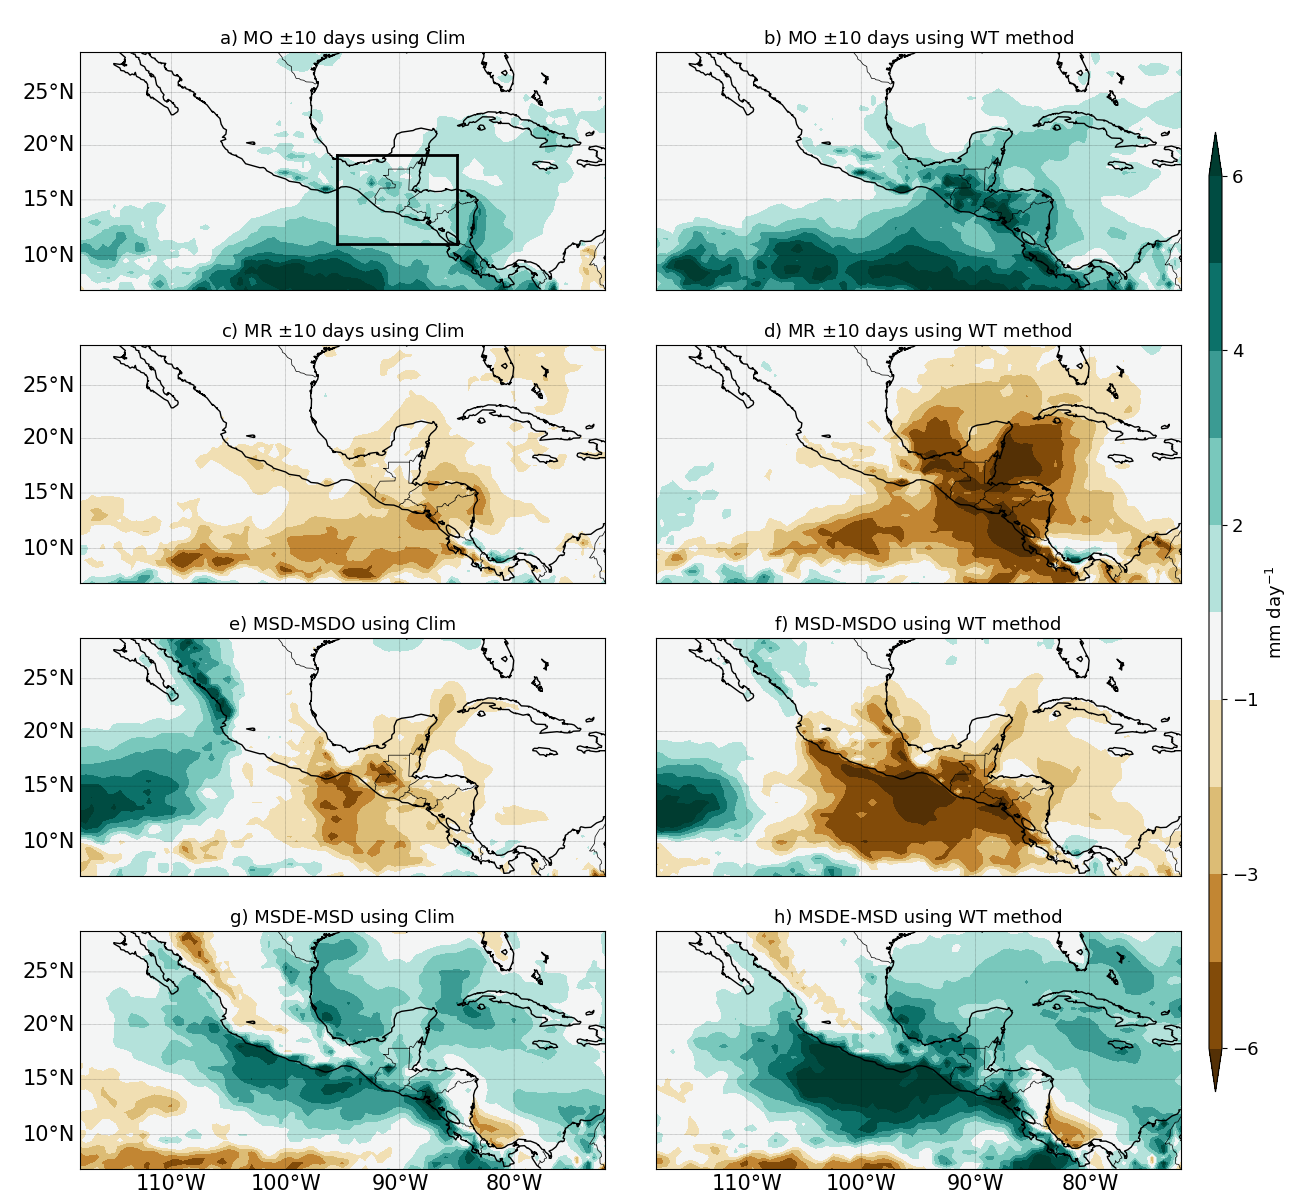
\includegraphics[width=0.95\linewidth]{figures/wav_fig10.png}
\caption[Precipitation anomalies after MSD]{  Precipitation anomalies for (a, b) the difference between the 10 days after monsoon onset and 10 days prior to onset (MO) using (a) the climatological dates of onset and (b) the dates estimated using the WT method. (c, d) are as in (a, b) but for monsoon retreat. (e, f) Difference between the Midsummer Drought (MSD) and the 10-day mean prior to the onset of the MSD (MSDO). (g, h) as in (e, f) but showing the difference between the end of the MSD (MSDE) and MSD. The data and calculations are from ERA-5. The black rectangle in a) shows the MSD area used to average the precipitation throughout this study.}
\label{fig:wav_fig11}
\end{figure}

Results from the application of the wavelet transform to the MSD, including the mean onset and retreat dates as well as the start and end dates of the MSD period, are reported in Table \ref{tab:4}.
The mean onset date in the observations is around pentad 27 (May 14), whereas the retreat date is around pentad 61 (October 31).
The end of the so-called first-peak period, or start of the relatively drier period (MSD), referred to in this thesis as MSD onset (MSDO) is consistently found in all the observed datasets to be around pentad 36 (around June 29).
The end of the drier period or start of the second peak, referred to in this thesis as MSD end (MSDE) is also consistently determined to be between pentads 48 to 49 in the four observational datasets.
In other words, the MSD has a mean duration of 12 pentads, or around two months, from late June to late August.
In the MOHC simulations, the MSD starts slightly later than observed by about two pentads, and ends about one pentad later than observed around September 10.

\begin{figure}[t!]
 \noindent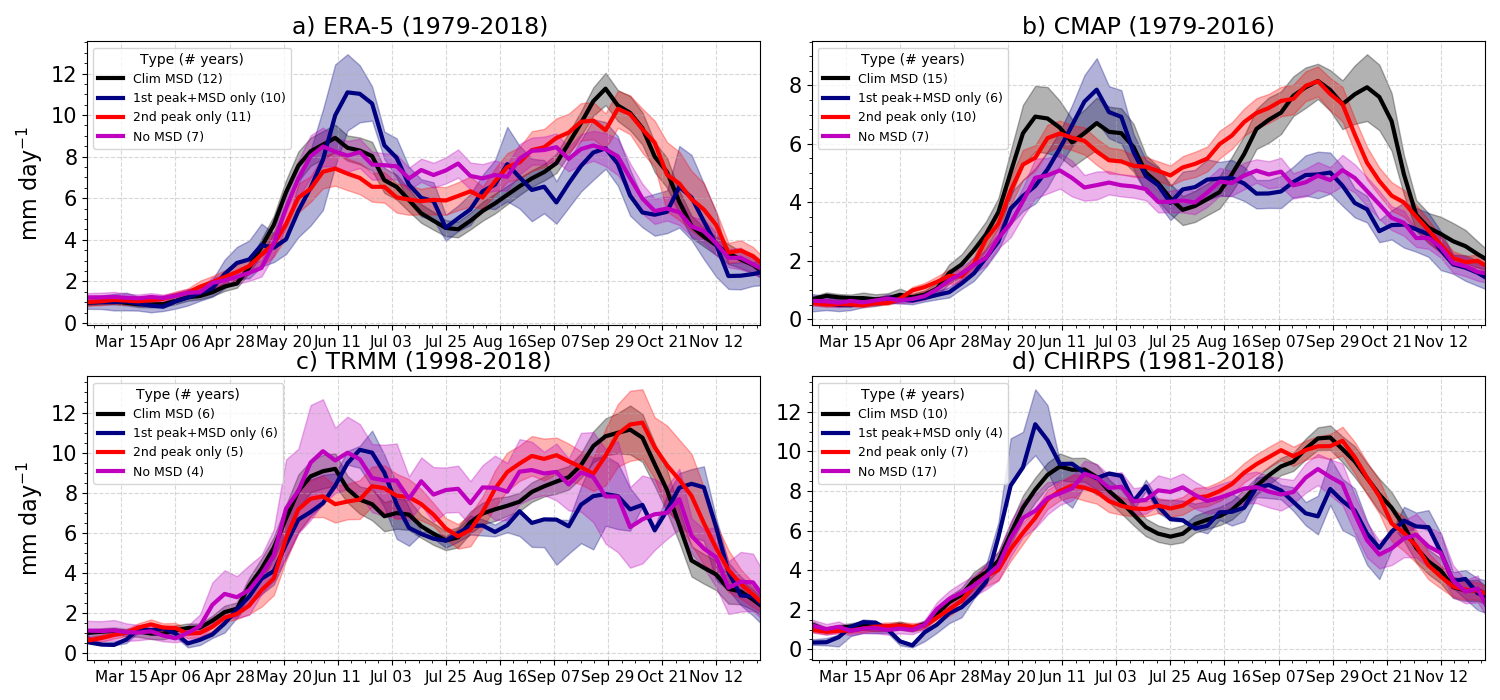
\includegraphics[width=\linewidth]{figures/wav_fig5c.png}
\caption[Seasonal cycle of precipitation for various MSD categories]{ Pentad-mean precipitation in years differentiated by MSD characteristics in four datasets: (a) ERA-5, (b) CMAP, (c) TRMM and (d) CHIRPS. The shading for each line represents first to third quantile of the distribution provided a bootstrapping with replacement all the years in each composite 10000 times.  }
\label{fig:S2}
\end{figure}
%\clearpage

Figure \ref{fig:wav_fig11} shows the rainfall anomalies associated with the different periods (stages) of the rainy season in southern Mexico and Central America. These include monsoon onset and retreat, and the start and end of the MSD, the MSDO and MSDE, respectively. For each stage, we compared the anomalies computed by separating the stages using the WT method or the dates of the climatological monsoon onset, retreat, MSDO and MSDE as found in Table \ref{tab:4}. In this way, the ability of the WT method to characterise rainfall variations is tested against a first best guess -- the climatological mean dates. 

Overall, using the dates for MSDO and MSDE from the climatological dates results in weaker anomalies than compositing via the specific dates for each year obtained with the WT method.  Even though the area-averaged signal used to diagnose the different MSD stages focuses on a small region of southern Mexico and northern Central America, the anomalies associated with the onset and end of the MSD (Figures \ref{fig:wav_fig11}f, h) extend across the East Pacific warm pool, most of the western coast of Mexico and into to the Caribbean Sea and Cuba. This result suggests that the MSD is part of a regional-scale process on the result of local-scale processes. 

The analysis of individual years of observed precipitation in the selected area-averaged time series showed that not all years showed a bimodal signal in the area-averaged precipitation (Fig. \ref{fig:S2}). In fact, a given year could be classified as having (1) a canonical two-peak structure separated by an MSD, (2) only having a first peak and an MSD but no second peak, (3) only having a second peak but no clear MSD or (4) a plateau-like monsoon season with no MSD-type variations (see Fig. \ref{fig:S2}). 


Due to this year-to-year variability in the characteristics of the seasonal cycle, an objective measure was defined to determine whether a signal presented a robust MSD-bimodal seasonal cycle.  
For this purpose, the WT algorithm was applied to randomly generated precipitation time series.
 The random time series are constructed by randomly sampling observations in the wet and dry seasons. 
 The pentad-mean onset and retreat dates from Table \ref{tab:4} were used to composite the observations into dry and wet distributions. 
 
 
 For a random time series that aims to mimic one year of precipitation, the rainfall values for each pentad in the year are randomly selected from the dry or wet distributions, depending on the pentad. In this way, the value of a given pentad of the random time series may have been observed at a different pentad; the only constraint is that the random values come from pentads that were observed in the same season: dry or wet. The logic behind this approach is that in most monsoon regions, the peak monsoon rainfall should follow a plateau, see for example the North and South American monsoons in Figure \ref{fig:8} in the previous chapter. However, a bimodal regime would show a notable decrease in precipitation in the middle of the rainy season, such that it cannot be explained by the inherent short-scale variability of rainfall. 
 
\begin{figure}[t!]
\centering
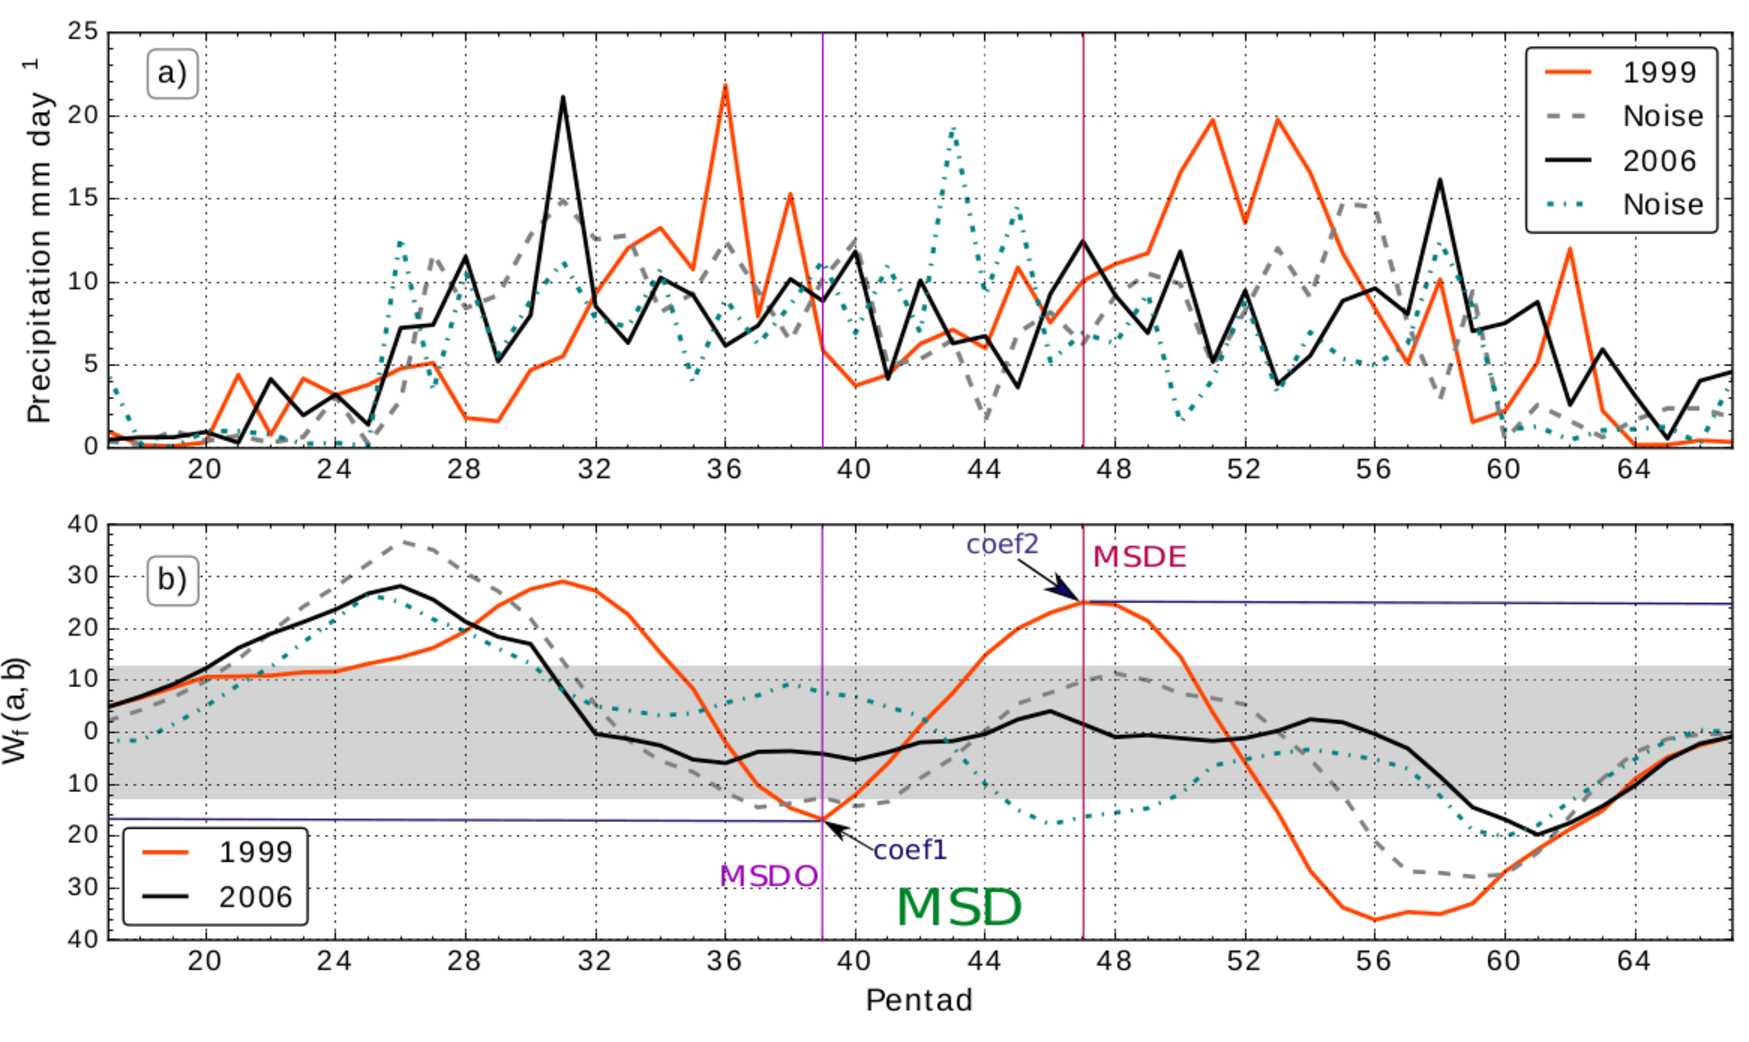
\includegraphics[width=\linewidth]{figures/wav_S1.pdf}
\caption[Determination of MSD timings and coefficients]{(a) Pentad-mean precipitation in two years of TRMM data: 1999 and 2006 and two randomly generated precipitation time series (see text). (b) Sum of the wavelet transforms of the time series in (a). The shaded region in gray in (b) corresponds to the interval between the first quantile of $coef1$ and the third quantile of $coef2$ of 10,000 random timeseries constructed with TRMM data. The onset (MSDO) and end (MSDE) of the relatively drier period, as well as the location and values of $coef1$ and $coef2$ for 1999 are labelled in (b). }
\label{fig:S1}
\end{figure}
 
 
 This approach has two advantages. First, that the random time series impose a monsoon-like feature with a sharp wet-dry season contrast but secondly, the random selection in the wet season removes the possible signal of the MSD in the climatological rainfall.
 The random time series are then constructed by randomly drawing values at each pentad  from the wet or dry season distributions of each dataset.
 Then, the WT method was used on 10,000 of these random-time series. This approach rendered a distribution of coefficients ($coef1$ and $coef2$) essentially representing the variability of the WT method applied to noise.
 
  Figure \ref{fig:S1} shows the pentad-mean time series from two years in the TRMM dataset, and two randomly generated time series.
The coefficients $coef1$ and $coef2$, illustrated in Figure \ref{fig:S1}b, measure the difference in precipitation between the first peak and the MSD period and the MSD and the second peak, respectively. The first quantile of $coef1$ and the third quantile of $coef2$ provide a measure of robustness for the observed $coef1$ and $coef2$. In other words, for a year to be classified as having a robust MSD signal, the resulting $coef1$ and $coef2$ of the WT procedure must be lower and higher, respectively, than those obtained for a random time series.
The analysis of $coef1$ then determines the existence of a first-peak MSD type variability and $coef2$ determines the robustness of a possible second-peak for that year.
By this procedure, a given year could fit into four categories:

\begin{itemize}
\item Canonical MSD: $coef1$ lower than the first quartile (25\%) of random $coef1$ and $coef2$ higher than the third quantile (75\%) of random $coef2$.
\item 1st peak+MSD: $coef1$ lower than the first quartile of random $coef1$ but $coef2$ lower than the third quartile of random $coef2$. In other words, the second peak is not distinguishable from noise.
\item 2nd peak only: $coef1$ higher than the first quartile of random $coef1$ but $coef2$ higher than the third quartile of random $coef2$. In other words, the second peak is distinguishable from noise, but there is no first-peak + MSD structure.
\item No MSD: $coef1$ higher than the first quartile of random $coef1$ and $coef2$ lower than the third quartile of random $coef2$. In other words, the precipitation time series shows no robust signal of an MSD regime, with a first or second peak.
\end{itemize}
 
\begin{figure}[t!]
\centering
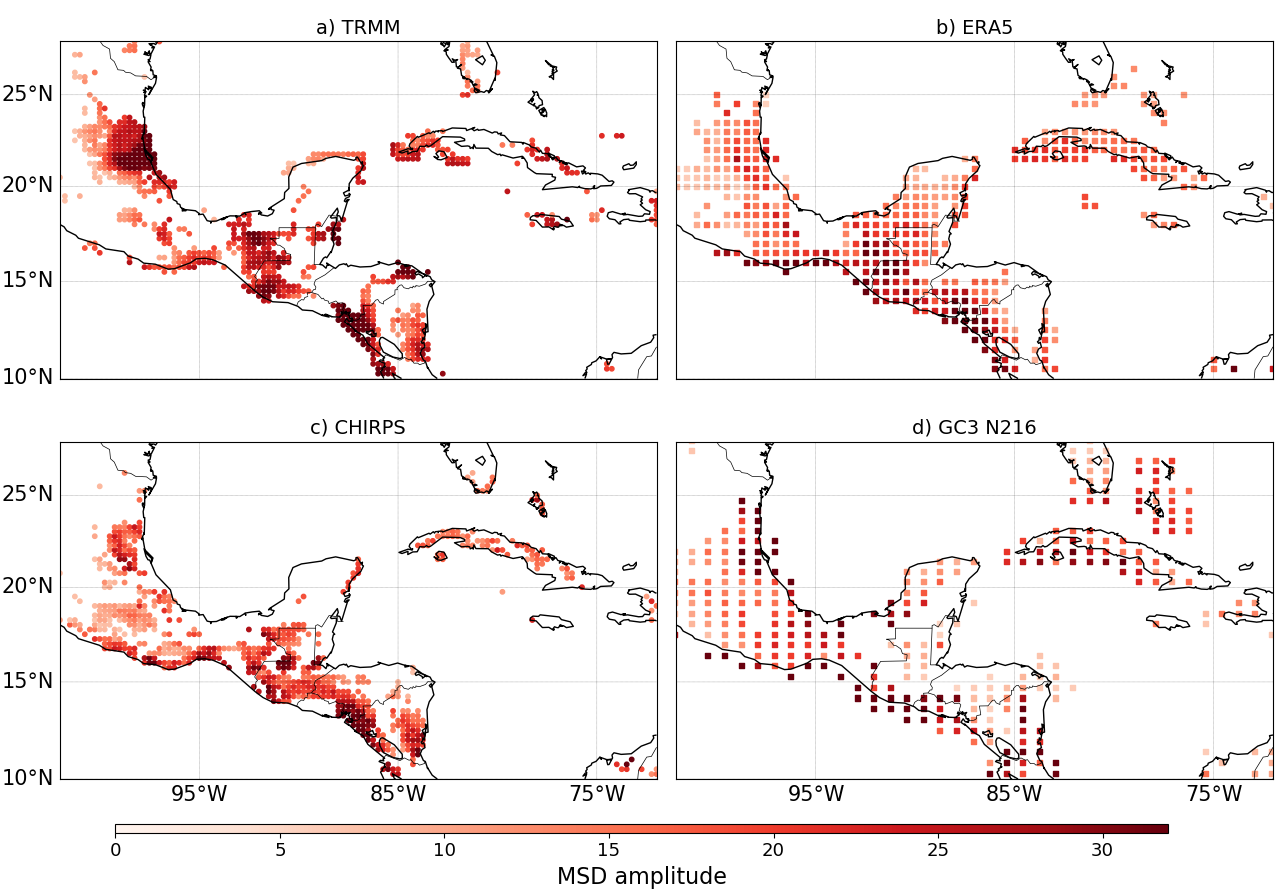
\includegraphics[width=\linewidth]{figures/wav_fig12.png}
\caption[Map of MSD significant regions]{Grid points where the MSD is significantly different, i.e.\, outside the first and second quartiles of the random distribution, from noise (see section 3.3) for a) TRMM, b) ERA-5, c) CHIRPS and d) GC3 N16-pi.  The magnitude of the MSD, measured as $coef2-coef1$ is shown in colour shading.  }
\label{fig:wavfinalmap}
\end{figure} 
 
 Figure \ref{fig:S2} shows how separating years into these categories affects the pentad-mean seasonal cycle of precipitation in southern Mexico and Central America in four observational datasets. This figure also validates the above procedure as the WT method is able to robustly separate years into the different categories. 

\begin{figure}[b!]
\centering
 %\noindent
 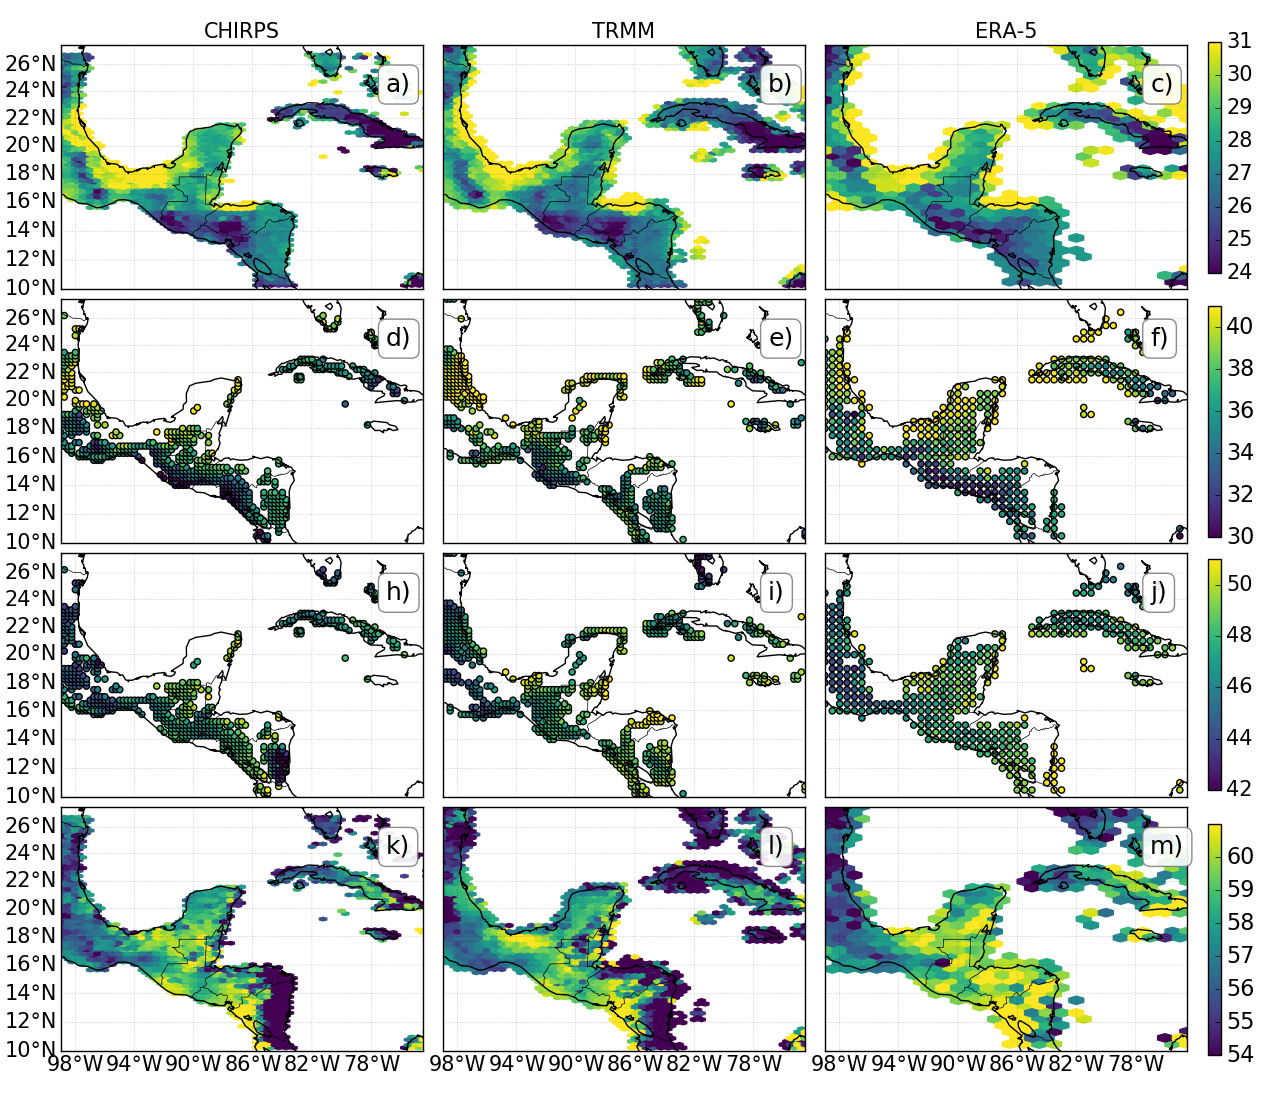
\includegraphics[width=\linewidth]{figures/wav_fig13.png}
\caption[Spatial distribution of MSD timings]{  Spatial distribution of pentad dates of the timings of the summer rainfall season in the MSD region, showing (a-c) MO dates and (d- f) MSDO dates, (g-i) MSDE and (j-l) MR for (left) CHIRPS, (middle) TRMM and (right) ERA-5. }
\label{fig:wav_fig13}
\end{figure}

For each dataset we determine those grid-points showing a robust MSD. We use the method outlined above to construct the random time series for each grid-point and estimate the random values of $coef1$ and $coef2$, repeating the procedure 10,000 times. A given grid-point is diagnosed to have a robust MSD when the value of $coef2-coef1$ is higher than the third quartile of the PDF of the random time series. The value of $coef2-coef1$ is a measure of the magnitude of the MSD since $coef2$ measures the relative strength of the second-peak compared to the MSD and therefore positive in an MSD grid-point and $coef1$ compares how dry the MSD is relative to the first-peak and thus negative if an MSD regime is observed at that grid point. 


Figure \ref{fig:wavfinalmap} shows the regions where the climatological rainfall shows a MSD signal that is distinguishable from noise, i.e., regions where the values of $coef2-coef1$ exceed the third quartile of the distribution composited with random time series, as well as the magnitude of the MSD for the TRMM, ERA5, CHIRPS and the GC3 N216 piControl simulation. Cuba, western Central America and most of southern and central-eastern Mexico exhibit a robust MSD signal. 
This map also shows that the strongest MSD signal is found on the western coast of northern Central America and northeastern Mexico. 
The high correspondence between the three observational datasets shows that the method is robust across datasets. These results agree well with previous studies on the spatial distribution of the MSD \citep{magana1999,perdigon2018,anderson2019multiscale,zhao2021}. In particular, the method is able to replicate the previously reported MSD signal in the Pacific Mexican coast and the stronger MSD signal in northeastern Mexico.  

Figure \ref{fig:wav_fig13} shows the spatial distribution of the mean onset and retreat pentads and the start and end of the MSD, in the grid-points where the signal is significant as in Fig. \ref{fig:wavfinalmap}. The earliest rainfall onset is found on the western coast of southern Mexico, Guatemala and El Salvador, as well as in Cuba, at pentad 25, whereas onset in the Yucatan peninsula is found at pentad 28 and even later, around pentad 31, in the eastern states of Mexico. In contrast, the retreat date seems spatially more homogeneous as northern Central American has a mean retreat date around pentad 59 and central Mexico around pentad 54.
The MSD coherently starts over the western coast of Guatemala and Chiapas around pentad 33. In contrast, the MSD on the eastern Mexican states of Veracruz and Campeche begins after pentad 40. The earliest MSD end (Figs. \ref{fig:wav_fig13}h-j) is found in central and northeastern Mexico, around pentad 42 whereas the MSD in Guatemala ends around pentad 48.



\section{Summary and discussion}

The assessment of the AMS in the MOHC submissions to CMIP6 in Chapter \ref{ch:4-ams} lacked a robust analysis of the representation of the timings of the monsoon. 
The principal reason for this shortcoming was the lack of a robust, widespread method to diagnose onset and retreat dates in the various regions of the AMS with the various datasets available. This chapter aimed to address this issue by developing a new method to compute onset and retreat dates for the purpose of intercomparison between multiple observational and model data.

The novel method described in this chapter uses pentad-mean precipitation data to compute a wavelet transform over multiple temporal scales from which a set of coefficients and diagnostics are used to determine onset and retreat dates. The wavelet function used is the Haar wavelet, a wavelet typically used to find abrupt changes in signals.
Onset is defined as the maximum of the sum of the coefficients of the wavelet transform computed over a range of temporal scales or dilations. These dilations were found to provide the best results in a range from 28 to 54 pentads. Monsoon retreat is similarly defined but uses the minimum of this sum of wavelet transform coefficients. The use of this method is illustrated using multiple observational datasets and climate model output. The method is compared to existing methods to find onset and retreat dates in three monsoon regions.

The method performs favourably to existing methods that use precipitation thresholds in the North American Monsoon, as shown by the anomalies of precipitation, wind and geopotential around the onset and retreat dates. 
The spatial distribution of monsoon onset and retreat in this region was found to be sensibly captured by the wavelet algorithm, illustrating the earlier onset in central-western Mexico and the later onset in northwestern Mexico, Arizona and New Mexico. 
The spatial distribution of onset and retreat dates was diagnosed to be very similar between the TRMM, CHIRPS and ERA5 datasets, which suggests that the method produces similar results in datasets with different resolutions and climatologies. These results confirm that these models reasonably simulate the seasonal cycle of precipitation in the North American monsoon. This result also suggests that the method is robust to be used at the grid-box scale, and not just for region-averaged time series.
 
The WT method also compares well to a hydrologically defined index (HOWI) in the Indian Monsoon, although the WT better captures the precipitation variations whilst HOWI betters captures changes to the moisture transport. However, the WT method is also able to capture strong differences in moisture transport around the onset and retreat dates, in both models and observations. The WT method obtains a later onset and retreat as compared to the HOWI index, which is possibly associated with a lag between the moisture transport about the Arabian Sea (as diagnosed by HOWI) and the precipitation over mainland India (as measured by the WT method). The spatial distribution of onset and retreat dates in the Indian Monsoon region, diagnosed using the WT method seems to be relatively consistent and coherent amongst the observational datasets, as the mean onset date in mainland India was found at pentad 32.
Onset is earliest on the western coast of India and the onset date appears to be very homogeneous in central India.

The WT method was extended to characterise the timings and strength of the Midsummer Drought (MSD), using the same principle as for determining onset in the Indian monsoon, but computing the WT over smaller dilations around the onset and retreat dates.  By using randomly-generated time series, the spatial distribution of grid-points displaying a robust MSD signal was found in Cuba, the northwestern coast of Central America and several regions of south and north-eastern Mexico.  The MSD in southern Mexico and northern Central America is found to start around pentads 35 and 36 (last week of June) and end around pentad 48 (mid-August) in most observational datasets and the ERA5 reanalysis. To our knowledge, this extension of the WT method provides one of the very few methods for characterising the MSD on sub-monthly scales.
%This method may be potentially useful when diagnosing changes to the characteristics of the MSD in models or observations, as will be shown in the following chapter. 


%discussion on problems with thresholds, 
%area-mean average 
%Current methods that diagnose monsoon onset and retreat using pentad or daily-mean precipitation time series are typically rigid threshold methods. These threshold methods depend on a number of parameters that need to be tuned for a specific monsoon region and for a specific dataset. 
%For instance, the method by \citetalias{geil2013} used a threshold value specific for the North American Monsoon and specific for the TRMM dataset but also to the limits of the area used for area-averaging the precipitation. In other words, the persistence and threshold values of most of the threshold methods require normalization, statistical treatment or additional tuning to the parameters to account for climatological differences in the datasets which introduces uncertainty. The method by \citetalias{arias2012} then uses a climatological mean value as the threshold, but in a climate model with a significantly positive bias in the dry winter season of a monsoon this method would be prone to error as the biased seasonal cycle may impose a biased calculation of monsoon onset and retreat. 

% different dataset climatology, characteristicis
% model climatology and biases. 
% window and persistence parameters vary monsoon region to another.


The WT method is in many ways similar to the agronomical and threshold methods \citep[e.g.][]{liebmann2001interannual,moron2014interannual}, as the implementation of the method uses a subjective determination of the dilation scales; these scales are comparable to the persistence and window parameters of the threshold methods. However, the WT method presented has three main advantages over most threshold methods. First, the method produces robust results for the Indian and North American monsoon of onset and retreat, and spatial distributions comparable to previous methods \citep{moron2014interannual} while not being subject to 'false hits' nor years without an identification of the onset and retreat dates. In other words, the method provides robust results without requiring further treatment of years with false hits or undetermined years. 

The second advantage of the method is portability, or utility, as the method shows robust and consistent results for three observational datasets, a reanalysis and climate model experiments with varying climate forcing but without any constraint or treatment of the data beforehand and in three different regions with different seasonal cycles. In other words, this method is robust across datasets and regions. In contrast to rigid threshold techniques \citep[e.g.][]{liebmann2001interannual}, the identification of onset and retreat for each time series, e.g. at each grid-point, is based upon coherent temporal changes within each precipitation time series while not using parameters determined \textit{a priori} specifically for a region. The WT method can then be used in any time series, regardless of the origin of the time series, without any further change or consideration than those established by the dilations scales determined in section 2.2.1. 
The portability of the method also means that the method can be implemented as a \textit{local-scale} method applied at the grid-box scale for high-resolution datasets such as CHIRPS as well as for regional scales using area-averaged time series.

Third, and in contrast to typical threshold methods, the wavelet method can be applied to climate model output straightforward using the same configuration of dilation scales, a feature of the method that is illustrated by our analysis of several experiments using the Hadley Centre models. The treatment of the data does not require  any normalisation or statistical treatment even when used for grid-point time series for different regions or experiments with varying forcing where the seasonal cycle or total annual rainfall may change notably within the model time series.


%This chapter follows up on some missing details of the previous chapter by analysing the timings  of the North American monsoon and the Central American MSD in the MOHC models by objectively computing the onset and retreat dates with the WT method. The results confirm that the CMIP6 MOHC models reasonably simulate the seasonal cycle of rainfall in North American monsoon and the MSD regions.
%Moreover, 

This chapter provides the main tool for the following chapter, which aims to better understand the physical mechanisms behind the MSD, a question that would be difficult to address without the existence of a robust method for determining the timings of the MSD at the pentad-scale.
